\section{Probability}\label{sec:probability_basics}
Here we consider a few rules of probability theory before we begin discussing Bayesian inference and hypothesis testing. We follow the guide of~\cite{wall2012practical} for the rules of probability. Firstly, for a given set of $N$ possible outcomes where each outcome has a probability $p_i$ of occurring then the sum of all possible outcomes must be unity. This can be expressed as
\begin{equation}
 \sum_{\limit i=1}^{\limit N} p_i = 1.
\end{equation}
This is also true for probability distribution functions $p(x)$ described by a continuous parameter $x$. We express this rule of probability as
\begin{equation}
 \int p(x) \, dx = 1.
\end{equation}

Next, we consider the probability of independent events occurring and the concept of conditional probability. Two events $A$ and $B$ are said to be independent of one another if the probability of $A$ is unaffected by what we may know about $B$. This can be stated as:
\begin{equation}\label{eq:prob_ind}
 p(A \, \mathrm{and} \, B) \equiv p(A, \, B) = p(A) \, p(B).
\end{equation}
In cases that independence does not hold we can consider the conditional probability of $A$ given the information that we know of $B$. This conditional probability is stated as
\begin{equation}
   p(A \, | \, B) = \frac{p(A, \, B)}{p(B)}.
\end{equation}
Here $p(A \, | \, B)$ is the probability of $A$ given that $B$ has occurred. If $A$ and $B$ are independent events this reduces back to Eq.~(\ref{eq:prob_ind}). If there are many possibilities for event $B$, which we label as $B_i$, then we can also attain the probability of $A$ through the following summation
\begin{equation}\label{eq:prob_marginalization}
   p(A) = \sum_{\limit i} p(A \, | \, B_i) \, p(B_i).
\end{equation}
This is called marginalization and pertains to summing out nuisance parameters. This technique of marginalization also generalizes to continuous probability distributions and can be expressed as
\begin{equation}
   p(A) = \int p(A \, | \, B) \, p(B) \, dB.
\end{equation}
In order to conduct Bayesian inference and hypothesis testing we will make extensive use of conditional probabilities and probability marginalization.

\section{Bayesian Inference}\label{sec:bayes_inf}
In Bayesian statistical inference we are interested in using our data to update our beliefs regarding hypotheses and the parameters that come with these hypotheses. We can make use of Bayes' theorem to take prior beliefs about hypotheses, take observations of the data, and use these observations to construct posterior beliefs about hypotheses. We begin this approach by introducing Bayes' theorem
\begin{equation} \label{eqn:BayesTheorem_basic}
     p(\mathrm{H}) \, p(\mathbf{d} \, |\, \mathrm{H})  =  p(\mathrm{H} \, | \, \mathbf{d}) \, p(\mathbf{d}).
\end{equation}
Here we have $p(\mathrm{H})$ which represents our prior belief about the hypothesis H. The likelihood $p(\mathbf{d} \, |\, \mathrm{H})$ represents the probability of observing our data under the assumptions implicity stated in our hypothesis H. We use these to update our inference on the probability of hypothesis H as expressed in the posterior probability $p(\mathrm{H} \, | \, \mathbf{d})$. Finally then we have $p(\mathbf{d}$, the probability of obtaining this data set. For the moment we will consider this as a normalization factor. For ease of reading we will change notation so that the prior $p(H)$ is $\pi (H)$, the likelihood $p(\mathbf{d} \, |\, \mathrm{H})$ is $\mathcal{L}(\mathbf{d} \, | \, \mathrm{H})$, the posterior distribution $p(\mathrm{H} \, | \, \mathbf{d})$ is $\mathcal{P}(\mathrm{H} \, | \, \mathbf{d})$, and the normalization factor $p(\mathbf{d})$ is $\mathcal{Z}(\mathbf{d})$ following the notation of~\cite{hobson2010bayesian}.

Within the context of parameter estimation we often use a hypothesis H that is composed from prior distributions on parameter values $\vec{\theta}$ that fully describe the hypothesis. In this context it is more helpful to rewrite Eq.~(\ref{eqn:BayesTheorem_basic}) as
\begin{equation}\label{eqn:BayesTheorem_PE}
   \mathcal{P}(\vec{\theta} \, | \, \mathbf{d}, \mathrm{H}) = \frac{\pi(\vec{\theta} \, | \, \mathrm{H}) \, \mathcal{L}(\mathbf{d} \, | \vec{\theta})}{\mathcal{Z}(\mathbf{d} \, | \, \mathrm{H})}.
\end{equation} 
In Eq.~(\ref{eqn:BayesTheorem_PE}) the normalization constant $\mathcal{Z}$ is often called the marginal likelihood since it marginalizes all parameters of the model H out of the likelihood~\cite{hobson2010bayesian}:
\begin{equation}\label{eqn:marg_likelihood}
    \mathcal{Z}(\mathbf{d} \, | \, \mathrm{H}) = \int \pi(\vec{\theta} \, | \, \mathrm{H}) \, \mathcal{L}(\mathbf{d} \, | \, \vec{\theta}) d\vec{\theta}.
\end{equation} 
This marginal likelihood is often called the evidence since it summarizes the likelihood of obtaining the data given the hypothesis over the entire prior distribution. That is, we have marginalized the likelihood across the entire prior distribution. We can compare the evidences between different hypotheses as a way to see which hypothesis better \textit{predicts} the data. The larger the evidence, the better the hypothesis predicts the data. In most practical cases this integral is analytically intractable due to the dimensionality of the prior distribution. We could consider estimation of this evidence via Monte Carlo sampling techniques. To clarify, we can consider Eq.~(\ref{eqn:marg_likelihood}) as the prior-weighted average likelihood.
We can consider a Monte Carlo simulation where we draw random samples from the prior distribution, measure the likelihood, and then take the arithmetic mean of this likelihood. This arithmetic mean will approximate the marginal likelihood up to some Monte Carlo uncertainty. In practice, this is impractical in realistic astrophysical applications~\cite{wall2012practical}. We will consider methods that are more effective for estimating the Bayesian evidence in Sections~\ref{sec:ti} and~\ref{sec:ssa}.

We can compare two competing hypotheses by calculating the likelihood ratio of the marginal likelihoods for each hypothesis. If the likelihood ratio is greater than unity, then the hypothesis in the numerator predicts the data with higher likelihood than the hypothesis in the denominator. If this likelihood ratio is smaller than unity, then the hypothesis in the numerator predicts the data with lower likelihood than the hypothesis in the denominator. This likelihood ratio test is known as the Bayes factor. For two hypotheses, $\mathrm{H}_A$, and $\mathrm{H}_B$, with marginal likelihoods $\mathcal{Z}(\mathbf{d} \, | \, \mathrm{H}_A)$ and $\mathcal{Z}(\mathbf{d} \, | \, \mathrm{H}_B)$, respectively, the Bayes factor is defined as
\begin{equation}
    \mathcal{B}^{\mathrm{H}_A}_{\mathrm{H}_B} \equiv \frac{\mathcal{Z}(\mathbf{d} \, | \, \mathrm{H}_A)}{\mathcal{Z}(\mathbf{d} \, |  \, \mathrm{H}_B)}.
\end{equation}
Therefore if the Bayes factor is unity for these two hypotheses, then each hypothesis is equally likely to have predicted the data. We can convert a Bayes factor into a posterior odds ratio to give the odds of one hypothesis over another via:
\begin{equation}\label{eqn:odds_ratio}
    \mathcal{O}^{\mathrm{H}_A}_{\mathrm{H}_B} = \mathcal{B}^{\mathrm{H}_A}_{\mathrm{H}_B} \times \frac{\pi(\mathrm{H}_A)}{\pi(\mathrm{H}_B)}.
\end{equation}
Here $\mathcal{O}^{\mathrm{H}_A}_{\mathrm{H}_B}$ represents the odds that hypothesis $\mathrm{H}_A$ is preferred over hypothesis $\mathrm{H}_B$ after the observation of the data. This is called the posterior odds ratio. The ratio $\pi(\mathrm{H}_A) / \pi(\mathrm{H}_B)$ represents our prior odds ratio, that is, how much more did we believe that hypothesis $\mathrm{H}_A$  was preferred over hypothesis $\mathrm{H}_B$  before observing the data. The prior odds ratio gives us a statement of what level of Bayes factor we would require before we begin to change our minds about the odds of hypothesis $\mathrm{H}_B$ being better supported in the data than hypothesis $\mathrm{H}_A$. It is considered good practice to state prior probabilities and prior odds at the outset of an experiment~\cite{hobson2010bayesian}. Choice of prior probabilities on hypotheses are subjective but should not be considered arbitrary since they represent explicit decisions in experimental design which requires scientific expertise. An uninformative prior on each hypothesis, indicating no prior preference for either hypothesis, would set the prior odds ratio to unity.

If there are only two hypotheses being considered then an odds ratio can be converted into a probability of one hypothesis over another hypothesis through the following expression~\citep{read2006encyclopedia}:
\begin{equation}\label{eqn:probability_odds_ratio}
    \mathcal{P} \left(\mathrm{H}_A \, | \, \mathbf{d}\right) = \frac{\mathcal{O}^{\mathrm{H}_A}_{\mathrm{H}_B}}{1 + \mathcal{O}^{\mathrm{H}_A}_{\mathrm{H}_B}}.
\end{equation}
Here the probability of hypothesis $\mathrm{H}_A$ after observation of the data is given as $\mathcal{P}(\mathrm{H}_A \, | \, \mathbf{d})$. This is the posterior probability of the hypothesis $\mathrm{H}_A$. Since there are only two possible hypotheses the posterior probability of $\mathrm{H}_B$ is $\mathcal{P}(\mathrm{H}_B)) \equiv 1 - \mathcal{P}(\mathrm{H}_A))$. In Fig.~\ref{fig:log_odds_v_probability} we compare the logarithm of the odds ratio with the posterior probability for a hypothesis. When the log odds ratio is $0$ the probability of one hypothesis relative to the other hypothesis is $0.5$. Furthermore, we can also make a mapping of this probability to a single-tailed z-score of a Gaussian distribution. This is the familiar test statistic $\sigma$ used in physics (see Chapter 2 for an example of its use for the estimation of the statistical significance of GW150914). Specifically, the conversion from probability to this statistic is given by $\mathrm{z-score} = -\sqrt{2} \mathrm{erfc}^{-1}(2p)$, where $\mathrm{erfc}^{-1}$ is the inverse complementary error function and $p$ is the probability value\footnote{In Chapter 2 we converted p-values to single-sided Gaussian standard deviation scores via the inverse error function. The formulation used here is equivalent.}. A z-score of $0$ ($0 \sigma$) indicates a $50\%$ probability, while a z-score of $5$ is $\sim$ $10^{-7}$ probability. The relationship between this z-score and the log odds ratio is shown in Fig~\ref{fig:log_odds_v_z_score}.

In cases where there are more than hypotheses available, we set one model as the fiducial model such that all Bayes factors are calculated relative to this fiducial hypothesis ($\mathrm{H}_{\mathrm{fiducial}}$)~\cite{read2006encyclopedia}. Then posterior probabilities for individual hypotheses can be calculated as
\begin{equation}\label{eqn:posterior_prob_multi}
    \mathcal{P} \left(\mathrm{H}_i \, | \, \mathbf{d}\right) = \frac{\mathcal{O}^{\mathrm{H}_i}_{\mathrm{H}_{\mathrm{fiducial}}}}
                                              {\sum^{\limit \mathrm{N}}_{\limit j=1} \mathcal{O}^{\mathrm{H}_j}_{\mathrm{H}_{\mathrm{fiducial}}}}.
\end{equation}
Here the summation is over all $N$ available hypotheses. This posterior probability for an individual hypotheses is often useful to calculate to compare how informative any individual hypothesis is relative to all available models. In practice can be computationally difficult to test a large set of hypotheses, but~\cite{ligo2019model} is an example of testing a large set of hypotheses in the field of gravitational wave astronomy.

As~\cite{read2006encyclopedia} notes we are often not just concerned with the Bayes factors and posterior probabilities on hypotheses but we also want to learn from the inference on parameters conditional on each of our tested hypotheses. We can inspect each of these posterior probabilities on parameters for each hypotheses in isolation or we can take a Bayesian model averaging approach of~\cite{kass1995bayes}. Bayesian model averaging involves coherently combining the parameter inference for common parameters from many different hypotheses. To do so we calculate the posterior probability for each hypothesis based on the posterior odds ratio (or Bayes factor if the prior odds ratios for hypotheses are unity) as in Eq.~(\ref{eqn:posterior_prob_multi}). Next, we reweight the marginal posterior probabilities for common parameters for each hypothesis by the posterior probability of the hypothesis. Finally, we sum these reweighted posterior probabilities on common parameters to create a multi-model parameter inference on these common parameters. This technique is often used in Bayesian cosmological modeling~\cite{hobson2010bayesian}. We mathematical expression for Bayesian model averaging for parameter inference on a parameter $\Delta$ can be stated as
\begin{equation}\label{eqn:BMA}
    \mathcal{P} \left( \Delta \, | \, \mathbf{d}\right) = \sum_{\limit i=1}^{\limit \mathrm{N}}  \mathcal{P} \left(\mathrm{H}_i \, | \, \mathbf{d}\right) \,  \mathcal{P} \left(\Delta \, | \, \mathbf{d}, \mathrm{H}_i\right).
\end{equation}
Here the summation is over all $N$ available hypotheses. The term $\mathcal{P} \left(\Delta \, | \, \mathbf{d}, \mathrm{H}_i\right)$ represents the parameter inference on $\Delta$ conditional on hypothesis $\mathrm{H}_i$. If we have a continuous ``hyper-parameter'' $\alpha$ that connects all the hypotheses we are testing then the summation in Eq.~(\ref{eqn:BMA}) becomes an integration over $\alpha$. 

In addition to testing hypotheses on one particular observation $\mathbf{d}$ it is possible to combine the inference from multiple observations, $\left\{\mathbf{d}_1, \mathbf{d}_2, \ldots, \mathbf{d}_\mathrm{N}\right\}$. If we are testing the same prior distribution and each observation is statistically independent, then the Bayes factor for multiple observations can be combined through multiplication~\cite{read2006encyclopedia, del2013demonstrating}. We temporarily suppress notation on hypotheses, and adopt the notation of~\cite{ly2018replication} for Bayes factors from multiple observations to give the combined Bayes factor as
\begin{equation}\label{eqn:multi_bayes_factors}
   \mathcal{B}(\mathbf{d}_1, \mathbf{d}_2, \ldots, \mathbf{d}_{\mathrm{N}}) = \mathcal{B}(\mathbf{d}_1) \times \mathcal{B}(\mathbf{d}_2) \times \ldots \times \mathcal{B}(\mathbf{d}_N). 
\end{equation}
Here $\mathcal{B}(\mathbf{d}_1, \mathbf{d}_2, \ldots, \mathbf{d}_{\mathrm{N}})$ represents the Bayes factor after many observations. Even if the Bayes factor for a particular hypothesis is not statistically significant for any individual observation $\mathbf{d}_i$, we can accumulate evidence over many observations to reach a clearer conclusion about how well supported a hypothesis is by the many observations.

We can also update our posterior distributions on parameters over many observations. Here we follow~\cite{dpac_technical} and consider the updated marginal posterior probability $\mathcal{P} \, \left(\Delta \, | \, \mathrm{H}, \mathbf{d}_1, \ldots, \mathbf{d}_N, \right)$ on a parameter $\Delta$ after $N$ observations
\begin{equation}
    \mathcal{P} \, \left(\Delta \, | \, \mathrm{H}, \mathbf{d}_1, \ldots, \mathbf{d}_N, \right) = \frac{\pi (\Delta \, | \, \mathrm{H} )}{c} \mathcal{L} (\mathbf{d}_1, \ldots, \mathbf{d}_N \, | \, \Delta , \mathrm{H}). 
\end{equation}
Here we have a prior $\pi (\Delta \, | \, \mathrm{H} )$ representing our belief on the parameter $\Delta$ over the entire collection of our observations. Our likelihood function $\mathcal{L}$ is separable if all events are statistically independent. In this case we can then write
\begin{equation}
    \mathcal{P} \, \left(\Delta \, | \, \mathrm{H}, \mathbf{d}_1, \ldots, \mathbf{d}_N, \right) = \frac{\pi (\Delta \, | \, \mathrm{H} )}{c} \mathcal{L} (\mathbf{d}_1  \, | \, \Delta , \mathrm{H}) \times \mathcal{L} (\mathbf{d}_2  \, | \, \Delta , \mathrm{H}) \times \ldots \mathcal{L} (\mathbf{d}_N  \, | \, \Delta , \mathrm{H}).
\end{equation}
Here we can substitute the likelihood $\mathcal{L}(\mathbf{d}_i  \, | \, \Delta , \mathrm{H})$, where $i$ marks the ith observation in the list of observations from $1$ to $N$, using Bayes' theorem. The likelihood can be substitute with the expression $\mathcal{P}' (\Delta \, | \, \mathbf{d}_i, \mathrm{H}) \, / \, \pi'(\Delta \, | \, \mathrm{H})$. We use a prime notation here on the marginal posterior distribution and marginal prior distribution on the parameter $\Delta$ to denote the distributions from observation of $\mathbf{d}_i$. Marginal posterior distributions on parameters can be approximated from an Monte Carlo simulation or a Markov-Chain Monte Carlo simulation. This procedure is generic and we can combine this result with the multi-model inference of Eq.~(\ref{eqn:BMA}) so that our parameter inference after $N$ observations is not completely dependent on any one particular parameter hypothesis.

We have so far treated the Bayesian evidence and Bayes factor as exact quantities that can be estimated exactly. We now consider error propagation and uncertainty estimation for Bayesian evidences and Bayes factors.

\section{Bayes Factor Uncertainty Estimation}\label{sec:practical_bayes}
When comparing hypotheses practically we must confront the fact that it is often too difficult to calculate the evidence analytically and so we often turn to Markov Chain Monte Carlo (MCMC) techniques to approximate the evidence~\cite{kass1995bayes, read2006encyclopedia, hobson2010bayesian, wall2012practical}. Since these methods are approximate it is useful to have some sense of the statistical or systematic uncertainties that arise from these MCMC methods\cite{hobson2010bayesian}. In our treatment we consider a model of the estimation of the logarithm of the evidence as a Gaussian distribution in log likelihood. This distribution has mean $\mu_{\widehat{\mathrm{ln} \, \mathcal{Z}}}$ representing a point estimate from the MCMC method, and standard deviation $\sigma_{\widehat{\mathrm{ln} \, \mathcal{Z}}}$ representing systematic or statistical uncertainties from the MCMC method. The logarithm of the evidence can be represented as 
\begin{equation}\label{eqn:p_log_z}
    p(\widehat{\mathrm{ln} \, \mathcal{Z}}) = \left(\frac{1}{\sqrt{2 \pi \sigma_{\widehat{\mathrm{ln} \, \mathcal{Z}}}}} \right) \mathrm{exp} \left \{-\frac{\left(\mathrm{ln} \, \mathcal{Z} - \mu_{\widehat{\mathrm{ln} \, \mathcal{Z}}}\right)^2} {2 \sigma_{\widehat{\mathrm{ln} \, \mathcal{Z}}}}  \right\}.
\end{equation}

The Bayes factor is the ratio of two evidences and hence the logarithm of the Bayes factor is the difference of the logarithms of two evidences. Here we suppress notation on hypothesis $\mathrm{H}_A$ and hypothesis $\mathrm{H}_B$, instead calling them $A$ and $B$, such that the logarithm of the Bayes factor can be expressed as
\begin{equation}\label{eqn:log_bayes_factor}
    \mathrm{ln} \, \mathcal{B}^A_B = \mathrm{ln} \, \mathcal{Z}_{\mathrm{A}} - \mathrm{ln} \, \mathcal{Z}_{\mathrm{B}}.
\end{equation}
However, since we treat $\mathrm{ln} \, \mathcal{Z}_{\mathrm{A}}$ as a random variable we must deal with the uncertainty in $\widehat{\mathrm{ln} \, \mathcal{Z}_{\mathrm{A}}}$. The logarithm of the Bayes factor then becomes the difference between two probability distribution functions. This can be solved via convolution and has been solved for the Gaussian case~\citep{bromiley2003products}. From \cite{bromiley2003products}, we can express $\widehat{\mathrm{ln} \, \mathcal{B}^A_B}$ as a Gaussian distribution function with mean $\mu_{\widehat{\mathrm{ln} \, \mathcal{B}^A_B}} = \mu_{\widehat{\mathrm{ln} \, \mathcal{Z}_A}} - \mu_{\widehat{\mathrm{ln} \, \mathcal{Z}_B}}$ and standard deviation $\sigma_{\widehat{\mathrm{ln} \, \mathcal{B}^A_B}} = \sqrt{\sigma_{\widehat{\mathrm{ln} \, \mathcal{Z}_A}}^2 + \sigma_{\widehat{\mathrm{ln} \, \mathcal{Z}_B}}^2 }$. This gives us the following expression for the distribution function on the logarithm of the Bayes factor:
\begin{equation}\label{eqn:p_log_b}
    p(\widehat{\mathrm{ln} \, \mathcal{B}^A_B}) = \left(\frac{1}{\sqrt{2 \pi \sigma_{\widehat{\mathrm{ln} \, \mathcal{B}^A_B}}}} \right) \mathrm{exp} \left \{-\frac{\left(\widehat{\mathrm{ln} \, \mathcal{B}^A_B} - \mu_{\widehat{\mathrm{ln} \, \mathcal{B}^A_B})}\right)^2} {2 \sigma^2_{\widehat{\mathrm{ln} \, \mathcal{B}^A_B}}}  \right\}.
\end{equation}

The expression in Eq.~(\ref{eqn:p_log_b}) is a Gaussian distribution function in $\widehat{\mathrm{ln} \, \mathcal{B}^A_B}$, but we often prefer to know the estimate on $\mathcal{B}^A_B$ and so we must use a transformation of coordinates. Rather than do this explictly we could recognize that Eq.~(\ref{eqn:p_log_b}) describes a log-normal distribution, which can be expressed as
\begin{equation}
    p(\widehat{\mathcal{B}^A_B}) = \frac{1}{\widehat{\mathcal{B}^A_B} \, \sigma_{\widehat{\mathrm{ln} \, \mathcal{B}^A_B}}} \frac{1}{2\pi} \mathrm{exp} \left \{-\frac{\left(\mathrm{ln} \, \widehat{\mathcal{B}^A_B} - \mu_{\widehat{\mathrm{ln} \, \mathcal{B}^A_B})}\right)^2} {2 \sigma^2_{\widehat{\mathrm{ln} \, \mathcal{B}^A_B}}}  \right\}.
\end{equation}
It is worth noting that for a sufficiently small standard deviation on the logarithm of the Bayes factor, the probability distribution function of the Bayes factor will look approximately Gaussian in shape. This log-normal Bayes factor distribution has a median value that is identical to the point-estimate Bayes factor, $\mathcal{B}^A_B = \mathrm{exp} \left[\mathrm{ln} \, \mathcal{Z}_{\mathrm{A}} - \mathrm{ln} \, \mathcal{Z}_{\mathrm{B}} \right]$. The expectation value (mean) of this log-normal distribution is always right of the median, while the mode of the distribution is always left of the median. Large standard deviations on the logarithm of the evidence will create very long tails for the distribution of the Bayes factor, which makes decision-making based on Bayes factors more risky. Studies that use this estimation of the Bayes factor should consider trying to limit the error on the logarithm of the evidence.

In Sec.~\ref{sec:bayes_inf} we gave an equation Eq.~(\ref{eqn:multi_bayes_factors}) for combining the Bayes factors from a series of observations. If we consider the logarithm of the Bayes factor from Eq.~(\ref{eqn:multi_bayes_factors}) then combining the combined logarithm of the Bayes factor is the sum of the logarithm of the Bayes factor from each observation. In this section we have modeled the logarithm of the Bayes factor as a Gaussian distribution, and so the combined logarithm of the Bayes factor across observations is the sum of a series of Gaussian distributions, which itself is a Gaussian distribution~\cite{bromiley2003products}. The combined logarithm of the Bayes factor across many observations is the Gaussian distribution described by
\begin{equation}
    p(\widehat{\mathrm{ln} \, \mathcal{B}^A_B}) \left(\mathbf{d}_1, \mathbf{d}_2, \ldots, \mathbf{d}_N \right) = \mathcal{N}\left(\mu = \sum \limits_{i=1}^{N} \mu_i, \, \, \sigma = \sqrt{\sum \limits_{i=1}^{N} \sigma_i^2}\right).
\end{equation} 
Here $p(\widehat{\mathrm{ln} \, \mathcal{B}^A_B}) \left(\mathbf{d}_1, \mathbf{d}_2, \ldots, \mathbf{d}_N \right)$ is the combined logarithm of the Bayes factor of hypothesis $A$ vs hypothesis $B$. Here $\mu_i$ is the point-estimate log-Bayes factor from observation $\mathbf{d}_i$, and $\sigma_i$ is the standard deviation of the log-Bayes factor from observation $\mathbf{d}_i$. If the $\mu_i$ and $\sigma_i$ are all comparable across observations, then we note that the mean value of the combined logarithm of the Bayes factor estimate tends to grow linearly for $N$ observations, while the standard deviation of the combined logarithm of the Bayes factor grows as $\sim \sqrt{N}$. And so, even if we cannot reduce $\sigma_i$ very well for individual observations $\mathbf{d}_i$, in the long-run of observations we may expect the combined logarithmic Bayes factor to tend in a direction of statistical significance where a decision on the hypothesis can be confidently made. If the combined logarithm of the Bayes factor constantly oscillates around $0$ over many observations then the error term $\sigma$ will overcome the mean-value $\mu$ and the log Bayes factor will have no utility in decision making.

To illustrate this growth in Bayes factor uncertainty we consider a toy-model where three estimators of the logarithm of the Bayes factor for hypothesis $\mathrm{H}_A$ and hypothesis $\mathrm{H}_B$. We denote these three log Bayes factor estimators as $\mathrm{E1}$, $\mathrm{E2}$, and $\mathrm{E3}$. We consider $400$ observations, where the true value of the log Bayes factor is $0.05$ for every observation. This is weak or anecdotal evidence for hypothesis $\mathrm{H}_A$ for each observation, but the evidence accumulates over several observations. After $400$ observations the combined log Bayes factor is $\400 \times 0.05 = 20$, which is a combined Bayes factor of $4.8 \times 10^8$. This would provide very large evidential support for hypothesis $\mathrm{H}_A$ (see Table~\ref{table:bayes_factor_interpretation} for rule-of-thumb statistical significance interpretation). The first Bayes factor estimator $\mathrm{E1}$ measures an unbiased estimate the log Bayes factor for each observation such that $\mu_i = 0.05$ and $\sigma_i = 0.05$. The second Bayes factor estimator $\mathrm{E2}$ also has an unbiased estimate the log Bayes factor for all observations such that $\mu_i = 0.05$, but has trouble getting a good error estimate, measuring with uncertainty $\sigma_i = 0.3$ in the log Bayes factor for each observation. Finally, the third Bayes factor estimator $\mathrm{E3}$ uses a method of Bayes factor estimation that is unintentionally biased such that they measure $\mu_i=0$ for all estimates, but their estimator gives a statistical uncertainty of $\sigma_i = 0.05$. Figure \ref{fig:LBFE} shows the behavior of these three Bayes factor estimators and their uncertainty at the $90 \%$ confidence interval. After $200$ observations, the true combined log Bayes factor is $10$, and so $\mathrm{E1}$ has estimated a combined log Bayes factor of ($8.8$, $10$, $11.2$), while $\mathrm{E2}$ has estimated a combined log Bayes factor of ($3$, $10$, $17$), and finally $\mathrm{E3}$ has estimated a combined log Bayes factor of ($-7$, $0$, $7$ )  at the ($5$th, $50$th, $95$th) percentiles respectively. Here, $\mathrm{E1}$ is the best estimator of the log Bayes factor, however $\mathrm{E2}$ also correctly follows positive support for hypothesis $\mathrm{H}_A$. We see that after $200$ observations $\mathrm{E3}$ has an unresolved Bayes factor with no evidential support for either hypothesis. The uncertainty confidence intervals for $\mathrm{E2}$ and $\mathrm{E3}$ still overlap however. After $400$ observations we find $\mathrm{E1}$ has measured ($18.3$, $20$, $21.6$), $\mathrm{E2}$ has measured ($29.9$, $20$, $10$), and $\mathrm{E3}$ has measured ($-9.9$, $0$, $9.9$). After $400$ observations, the $90 \%$ confidence intervals of $\mathrm{E2}$ and $\mathrm{E3}$ no longer overlap. We also find that $\mathrm{E1}$ and $\mathrm{E2}$ have decisive levels of statistical significance to give support to hypothesis $A$. Meanwhile, $\mathrm{E3}$ has accumulated no relative evidence between hypotheses and the uncertainty in the logarithm of the Bayes factor has become extremely large. 

If we want to use Bayes factors to make decisions on the credibility of hypotheses in gravitational wave astronomy we should use the most accurate and unbiased methods for their estimation. Reducing the bias and variance of our Bayes factor estimators will play an important role in our ability to discriminate theories in physics that are supported by the data from those that are not. We now move on to practical methods for estimating the Bayesian evidence, Bayes factors, and their uncertainties via Markov-Chain Monte Carlo methods.

\section{The Thermodynamic Integration Method for Estimating the Bayesian Evidence}\label{sec:ti}
The first Markov-Chain Monte Carlo (MCMC) method that we consider for Bayesian hypothesis testing is the thermodynamic integration method. Many MCMC samplers use a chain of multiple temperatures to simulate annealing as a means for gradually guiding the MCMC sampler from the prior distribution to the posterior distribution~\citep{emcee, vousden:2016, doi:10.1143/PTPS.157.317, B509983H}. These multiple temperatures are helpful for finding the global maxima and modes of the posterior distribution. In addition to finding the modes of the posterior distribution, this method is also useful for estimating the logarithm of the evidence. We focus on the importance of thermodynamic integration for the estimation of the logarithm of the evidence. In particular we follow the of~\cite{lartillot2006computing, friel2008marginal} which is called the method of power-posteriors. In this method, each temperature describes a tempered posterior distribution. These tempered posterior distributions are called power-posterior because they can be expressed as
\begin{equation}
    \mathcal{P}\left(\vec{\theta}|\mathbf{d}, H\right)_\beta \propto \pi\left(\vec{\theta} | H\right) \mathcal{L}\left(\mathbf{d} | \vec{\theta}, H\right)^\beta.
\end{equation}\label{eq:power_posterior}
Here $\mathcal{P}\left(\vec{\theta}|\mathbf{d}, H\right)_\beta$ is the power-posterior. The likelihood is raised to the power of the inverse-temperature $\beta$. The prior distribution is left identical to the standard, untempered prior distribution usesd in hypothesis testing and paramter inference. For a value of $\beta$ = $0$ the power-posterior is equivalent to the prior distribution, while for a value of $\beta$ = $1$ the power-posterior is equivalent to the posterior distribution. The normalization constant for the power-posterior in Eq.~(\ref{eq:power_posterior}) is the normalizing constant for that power-posterior, given as $\mathcal{Z}(\mathbf{d} \, | \ ,H)_\beta \equiv \int \pi\left(\vec{\theta} \, | \, \mathrm{H}\right) \mathcal{L}\left(\mathbf{d} | \vec{\theta}, \mathrm{H}\right)^\beta d\vec{\theta}$.

From these power-posterior distributions we can use a thermodynamic integration method~\citep{lartillot2006computing,friel2008marginal} to estimate the logarithm of the evidence. For the derivation of this thermodynamic integration method we follow \citep{annis2019thermodynamic}.
We begin by considering the following expression implied by the 2nd Fundamental theorem of Calculus:
\begin{equation}\label{eqn:ti_identity}
    \mathrm{ln} \, \mathcal{Z}_{\beta=1}\left(\mathbf{d}\right) - \mathrm{ln} \, \mathcal{Z}_{\beta=0}\left(\mathbf{d}\right) = \int^1_0 \left(\frac{d\left(\mathrm{ln} \, \mathcal{Z}_\beta \left(\mathbf{d}\right) \right)}{d\beta}\right) \, d\beta = \int^1_0 \frac{1}{\mathcal{Z}_\beta \left(\mathbf{d}\right)} \frac{d \, \mathcal{Z}_\beta \left(\mathbf{d}\right)}{d\beta} d\beta.
\end{equation}
For a properly normalized prior, $\pi(\vec{\theta}$, $\mathrm{ln} \, \mathcal{Z}_{\beta=0} \left(\mathbf{d}\right) = 0$. This leaves the marginal likelihood at $\beta=1$ that we are interested in which is the untempered $\mathrm{ln} \, \mathcal{Z} \left(\mathbf{d}\right)$. Now we can expand Eq.~(\ref{eqn:ti_identity}) as:
\begin{equation}
    \mathrm{ln} \, \mathcal{Z} \left(\mathbf{d}\right) = \int_0^1 \frac{\int \frac{d}{d\beta} \left[\pi\left(\vec{\theta}\right) \, \mathcal{L} \left(\mathbf{d}|\vec{\theta} \right)^\beta \right]\, d\vec{\theta} d\vec{\theta}}{\int \pi\left(\vec{\theta}\right) \, \mathcal{L}\left(\mathbf{d}|\vec{\theta} \right)^\beta \, d\vec{\theta}}.
\end{equation}\label{eqn:ti_ref1}
Suppressing notation on $\theta$ and $\mathbf{d}$, for clarity, we the derivative in the numerator of Eq.~(\ref{eqn:ti_ref1}) to get:
\begin{equation}
    \mathrm{ln} \, \mathcal{Z} = \int^1_0 \frac{\int \pi \, \, \, \left(\mathrm{ln} \, \mathcal{L}\right) \, \, \, \mathcal{L}^{\beta} d\theta}{\int \pi \mathcal{L}^{\beta} d\theta} d\beta.
\end{equation}
Using Bayes' theorem we can replace the numerator and denominator with $\mathcal{P}_\beta = \pi \mathcal{L}^\beta \, / \, \mathcal{Z}_\beta$ to get:
\begin{equation}
    \mathrm{ln} \, \mathcal{Z} = \int^1_0 \frac{\int \mathcal{P}_\beta \, \left(\mathrm{ln} \, \mathcal{L}\right) d\theta}{\int \mathcal{P}_\beta   d\theta} d\beta.
\end{equation}
This simplifies to:
\begin{equation}
   \mathrm{ln} \, \mathcal{Z} = \int^1_0 \langle \mathrm{ln} \, \mathcal{L} \rangle_{\mathcal{P}_\beta} \, d\beta.
\end{equation}\label{eq:thermoint}
Therefore, the logarithm of the evidence is given by the one dimensional integral in Eq.~(\ref{eq:thermoint}).
Here $\langle \mathrm{ln} \, \mathcal{L} \rangle_{\mathcal{P}_\beta}$ represents the average untempered log-likelihood under the measure described by the power-posterior distribution at $\beta$. This is the average untempered log likelihood when drawing random samples from the power-posterior distribution at $\beta$. We suppress this notation to write $\langle \mathrm{ln} \, \mathcal{L} \rangle_{\mathcal{P}_\beta} \equiv \langle \mathrm{ln} \, \mathcal{L} \rangle_\beta$. With the thermodynamic integration method we have reduced a potentially large $N$ dimensional integral into a one dimensional integral. This method is an ubiased estimator of the logarithm of the evidence provided that samples of $\langle \mathrm{ln} \, \mathcal{L} \rangle_\beta$ can be drawn in an unbiased manner from power-posteriors~\citep{carlson2016partition}.

It is also convenient to describe additional derivatives of the thermodynamic integrand. In general, $\mathrm{n}^{\mathrm{th}}$ derivatives of the form $\mathrm{ln} \, \mathcal{Z}$ can be solved by referring to Eq.~$0.435$ of~\cite{gradshteyn2015table}\footnote{Note that the solution in~\cite{gradshteyn2015table} has a minor typo, which we correct here.}:
\begin{equation}\label{eqn:gradshteyn_derivatives}
    \frac{d^n}{d\beta^n}\left( \mathrm{ln} \, \mathcal{Z} \right) = \sum_{k=1}^{n} \frac{(-1)^{(k+1)} {{n}\choose{k}}}{k \mathcal{Z}^k} \frac{d^n}{d\beta^n} \left(\mathcal{Z}^k\right).
\end{equation}
The first derivative, $n=1$, we have already solved as $\langle \mathrm{ln} \, \mathcal{L} \rangle_\beta$. The next derivative, $n=2$, was found in~\cite{friel2014improving} as $\mathrm{Var}(\mathrm{ln} \, \mathcal{L})_\beta$ = $\langle (\mathrm{ln} \, \mathcal{L})^2\rangle_beta - \langle \mathrm{ln} \, \mathcal{L} \rangle^2_\beta$. This is the variance of the untempered log likelihood samples when drawn from the power-posterior at $\beta$. We solve the next derivative, $n=3$, as:
\begin{equation}\label{eqn:third_ti_deriv}
    \frac{d^3}{d\beta^3}\left( \mathrm{ln} \, \mathcal{Z}\right) = \langle \left(\mathrm{ln} \, \mathcal{L} \right)^3\rangle_\beta + 2 \langle \mathrm{ln} \, \mathcal{L} \rangle^3_\beta - 3 \langle \left(\mathrm{ln} \, \mathcal{L} \right)^2\rangle_\beta \langle \mathrm{ln} \, \mathcal{L}\rangle_\beta.
\end{equation}
In practice, we have found this third derivative in Eq.~(\ref{eqn:third_ti_deriv}) is not computationally stable in our applications in gravitational wave astronomy where the log likelihood can be $\sim\mathcal{O}(10^{-7}$. However, we observe that the pattern of the nth derivative of $\mathrm{ln} \, \mathcal{Z}$ with respect to $\beta$ follows the pattern of the nth cumulant~\citep{kardar2007statistical} of the power-posterior distribution at $\beta$~\cite{carlson2016partition}. See Table~\ref{table:cumulants} for examples up to the $4$th derivative. In fact, $\mathcal{Z}$ is analagous to a partition function in Bayesian statistical inference~\citep{carlson2016partition, lamont2019correspondence}. This cumulant property is helpful because it can make computation of values of higher order derivatives more numerically stable since cumulants of order $\ge 2$ are shift-invariant~\cite{kardar2007statistical}. We can make the transformation of variables, $\widetilde{\mathrm{ln} \, \mathcal{L}} \equiv \mathrm{ln} \, \mathcal{L} - \mathrm{ln} \, \mathcal{L}_{\mathrm{max}}$ for every power-posterior before computing the numerical value of higher order derivatives of $\mathrm{ln} \, \mathcal{Z}$. We have tested this transformation rule on higher order derivatives and found it to be both accurate and numerically stable, confirming the cumulant properties of the derivatives. However, we have also found that the samples drawn from power-posterior simulation using the parallel-tempered \emph{emcee} sampler~\citep{emcee,vousden:2016} may not be accurate enough to permit accurate calculation of derivatives higher than order $3$ in all cases.

In Fig.~\ref{fig:gooseneck_linear} we show the thermodynamic integrand and the next two derivatives for a gravitational wave analysis that uses $51$ temperatures. We also show the thermodynamic integrand and the next two derivatives on a logarithmic scale in $\beta$ in Fig.~\ref{fig:gooseneck_log} so that the curvature of the thermodynamic integrand is easier to see. In practice, plots like Figs.~\ref{fig:gooseneck_linear}, \ref{fig:gooseneck_log} are helpful to inspect for places where the integrand may not be well sampled in $\beta$ and hence require additional inverse-temperatures~\cite{liu2016evaluating, de2011free, de2013comparison} for an accurate estimate of the logarithm of the evidence. Of particular note is the instability in the middle (bottom) subplot of Fig.~\ref{fig:gooseneck_log} where the second (third) derivative is not perfectly smooth in $\beta$. We expect the thermodynamic integrand to be smooth and monotonically increasing as $\beta$ goes from $0$ to $1$~\cite{annis2019thermodynamic}. In Fig.~\ref{fig:gooseneck_linear} there is some numerical instability at $\beta \sim 10^{-9}$. The other derivatives of the thermodynamic integrand should also be smooth. This instability implies, the need for a better tempering sampler or bias-corrective terms in the sampling such as those found in the multi-tempering samplers of~\cite{oates2017control,evans2019thermodynamic}. The instability in Figs.~\ref{fig:gooseneck_linear}, \ref{fig:gooseneck_log} is very slight however and we would not expect an effect like this to significantly impact the Bayes factor estimation.

After inspection that the MCMC sampler has produced a smooth and well-behaved thermodynamic integrand we can use numerical quadrature routines to integrate the thermodynamic integrand with respect to $\beta$. In Section~\ref{sec:ti_num_quad} we describe different polynomial-based quadrature integration techniques for computing the thermodynamic integral from a finite set of inverse-temperatures $\beta$.

\subsection{Numerical Quadrature}\label{sec:ti_num_quad}
The thermodynamic integral in Eq.~(\ref{eq:thermoint}) can be estimated through numerical quadrature rules such as the trapezoidal rule or Simpson's rule. Since optimal placements of inverse-temperatures $\beta$ are not typically uniformly distributed between $0$ and $1$~\cite{annis2019thermodynamic}, it is helpful to consider integration rules that do not depend on equally spaced abscissa ($\beta$ in the context of thermodynamic integration). A polynomial interpolant that does not make of equally spaced abscissa is the Newton's divided difference polynomial, see~\cite{brun1953generalization, selmer1958numerical, abramowitz1965handbook} for how to construct these polynomials. We can then integrate these interpolants to create numerical quadrature rules.

First we consider the trapezoidal rule which in the context of thermodynamic integration is
\begin{equation}
    \widehat{\mathrm{ln} \, \mathcal{Z}}_{\mathrm{Trapz}} = \sum_{i=0}^{N_\beta-1} \frac{1}{2} \left(\beta_{i+1} - \beta_i \right) \left(\langle \mathrm{ln} \, \mathcal{L} \rangle_{\beta_{i+1}} + \langle \mathrm{ln} \, \mathcal{L} \rangle_{\beta_{i}} \right)
\end{equation}
Here $N_\beta$ represents the number of $\beta$ being summed over in the integration estimation. The error correction term to the trapezoidal rule can be found by integrating the next-to-leading order Taylor polynomial~\citep{abramowitz1965handbook}, yielding:
\begin{equation}
    \widehat{\mathrm{ln} \, \mathcal{Z}}_{\mathrm{Trapz \, +}} \approx \widehat{\mathrm{ln} \, \mathcal{Z}}_{\mathrm{Trapz}} + \sum_{i=0}^{N_\beta-1} -\frac{1}{12} \left(\beta_{i+1} - \beta_i \right)^2 \left[f'(\beta_{i+1}) - f'(\beta_{i}) \right].
\end{equation}
Here $f'(\beta_i)$ represents the second derivative of $\mathrm{ln} \, \mathcal{Z}$ with respect to $\beta$. It was found in~\cite{friel2014improving} that this corresponds to the variance of the untempered log likelihood as drawn from the power-posterior at $\beta_i$.

Simpson's rule for unequally spaced abscissa under Newton's divided difference interpolation~\citep{easa1988area} is:
\begin{equation}
    \widehat{\mathrm{ln} \, \mathcal{Z}}_{\mathrm{Simps}} = \sum_{\mathrm{i\, is\, even}, \, \, i=0}^{N_\beta-2} \frac{h_i + h_{i+1}}{6} \left [ A \, \langle \mathrm{ln} \, \mathcal{L} \rangle_{\beta_{i}} + B \, \langle \mathrm{ln} \, \mathcal{L} \rangle_{\beta_{i+1}} + C \, \langle \mathrm{ln} \, \mathcal{L} \rangle_{\beta_{i+2}}\right ],
\end{equation}
for the expressions:
\begin{equation}
\begin{array}{lll}
     A &= \left [(2h_i - h_{i+1})\right] \, / \, h_i, \\ \\ 
     B &= \left [(h_i+h_{i+1})^2 \right] \, / \, \left[h_i h_{i+1}\right], \\ \\
     C &= \left [(2h_{i+1} - h_i)\right] \, / \, h_{i+1}. \\ \\
\end{array}
\end{equation}
Here  $h_i \equiv \beta_{i+1} - \beta_i$, and $h_{i+1} \equiv \beta_{i+2} - \beta_{i+1}$. The error corrective term for Simpson's rule can thus be solved in the same manner as for the trapezoidal rule and we find:
\begin{equation}
    \widehat{\mathrm{ln} \, \mathcal{Z}}_{\mathrm{Simps \, +}} \approx \widehat{\mathrm{ln} \, \mathcal{Z}}_{\mathrm{Simps}} + \sum_{\mathrm{i\, is\, even}, \, \, i=0}^{N_\beta-2} \frac{1}{72}\left(\beta_{i+2} - \beta_{i} \right)^2 (\beta_i - 2\beta_{i+1} + \beta_{i+2})\frac{f''(\beta_{i+2}) - f''(\beta_i)}{\beta_{i+2} - \beta_i}.
\end{equation}
Here $f''(\beta_i)$ represents the third derivative of $\mathrm{ln} \, \mathcal{Z}$ with respect to $\beta$, which is in Eq.~(\ref{eqn:third_ti_deriv}).

The cubic integration rule for unequally spaced abscissa under Newton's divided difference interpolation can be found in~\cite{brun1953generalization,selmer1958numerical,chambers1989estimating} or can be derived through the tools in~\cite{abramowitz1965handbook}. We present the form given in~\cite{chambers1989estimating}:
\begin{equation}
    \widehat{\mathrm{ln} \, \mathcal{Z}}_{\mathrm{cubic}} = \sum_{\mathrm{i\, is\, a \, multiple \, of \, 3}, \, i=0}^{N_\beta-3} \frac{h_i + h_{i+1} + h_{i+2}}{12} \left [A \, \langle \mathrm{ln} \, \mathcal{L} \rangle_{\beta_{i}} + B \, \langle \mathrm{ln} \, \mathcal{L} \rangle_{\beta_{i+1}} + C \, \langle \mathrm{ln} \, \mathcal{L} \rangle_{\beta_{i+2}} + D \, \langle \mathrm{ln} \, \mathcal{L} \rangle_{\beta_{i+3}}\right ],
\end{equation}
for expressions:
\begin{equation}
\begin{array}{llll}
     A &= \left [3h_i^2 -h_{i+1}^2 +h_{i+2}^2 +2 h_i h_{i+1} - 2h_i h_{i+2}\right] \, / \, \left [h_i (h_i + h_{i+1}) \right ], \\ \\
     B &= \left [(h_i + h_{i+1} + h_{i+2})^2 (h_i + h_{i+1} - h_{i+2})\right ]  \, / \, \left[h_{i} h_{i+1} (h_{i+1} h_{i+2})\right ], \\ \\
     C &= \left [(h_i + h_{i+1} + h_{i+2})^2 (h_{i+1} + h_{i+2} - h_i)\right ] \, / \, \left [ h_{i+1} h_{i+2} (h_i + h_{i+1}) \right], \\ \\
     D &= \left [ h_i^2 - h_{i+1}^2 +3 h_{i+2}^2 - 2h_i h_{i+2} + 2 h_{i+1} h_{i+2}\right ] \, / \, \left [h_{i+2}(h_{i+1} + h_{i+2}) \right].\\ \\
\end{array}
\end{equation}
Here we have defined $h_i \equiv \beta_{i+1} - \beta_{i}$, $h_{i+1} \equiv \beta_{i+2} - \beta_{i+1}$, and $h_{i+2} \equiv \beta_{i+3} - \beta_{i+2}$.

We recommend caution in using the thermodynamic integral through a higher order polynomial quadrature rule as the integrand may not be well interpolated by higher order polynomials. Additionally, higher order cumulants are difficult to estimate from sampled data~\cite{kardar2007statistical}. Thus there may be very little incentive for going to higher order polynomial rules as improved accuracy is not always guaranteed by going to higher order polynomial integration rules~\citep{epperson1987runge}. Since the true value of the logarithm of the evidence is not usually known we recommend comparing the estimates from all available quadrature rules to ensure consistency.

Future studies may make use of quadrature rules from Taylor series polynomial interpolants for unequally spaced abscissa, from ratios of Taylor series polynomials through the Pad$\textrm{\'e}$ approximant~\citep{press1992pade}, or other interpolant functions. Improvement in numerical integration for thermodynamic integration may also be improved by focusing on increasing the number of inverse-temperatures $\beta$ and by improved placement of $\beta$.

\subsection{Monte Carlo Error Estimation}
Here we follow the discussion from~\cite{annis2019thermodynamic} for estimating the Monte Carlo error in the thermodynamic integral under a generic quadrature rule. The Monte Carlo error for thermodynamic integration is the uncertainty in the estimate of the integral due to only having a finite set of samples from a Markov-Chain Monte Carlo simulation. This uncertainty enters into the integration as an uncertainty in the $\langle \mathrm{ln} \, \mathcal{L} \rangle$. The variance of the thermodynamic integral estimator, $\widehat{\mathrm{ln} \, \mathcal{Z}}$, from Monte Carlo error can be found in two steps. First, calculate the thermodynamic integral for each sample of untempered log likelihoods drawn from the power-posterior at $\beta$. For $N$ samples drawn from each power-posterior this generates $N$ thermodynamic integral values. The quadrature rule for the integration is generic; we can use the trapezoidal rule, Simpson's rule, etc. From these $N$ integral values we take the sample variance and then divide by the number of samples $N$ to generate an estimate of the population variance of the thermodynamic integration. This population variance of the logarithm of the evidence represents a long-run estimate of the variance of the estimator. This variance can be represented as:
\begin{equation}
    \sigma^2_{\mathrm{MC}} = \frac{1}{N} \sigma^2_{\mathrm{sample}}.
\end{equation}
Here, $\sigma^2_{\mathrm{MC}}$ represents the Monte-Carlo variance for the thermodynamic integration estimator while $\sigma^2_{\mathrm{sample}}$ is the sample variance and $N$ represents the number of available samples. This $\sigma^2_{\mathrm{MC}}$ can be seen as the standard error of the mean value of the logarithm of the evidence due to Monte Carlo uncertainty. See Fig.~\ref{fig:ti_monte_carlo_error} for a visualization of this procedure.

Repeated runs where the random seed for the MCMC analysis was changed has shown that the variance estimate from presented in~\cite{annis2019thermodynamic} is a plausible confidence interval estimate for Monte Carlo error.

\subsection{Convergence Error Estimation}\label{sec:evidence_convergence}
The procedure for estimating the marginal likelihood from power-posterior simulation requires that the power-posteriors all converge to a final stationary distribution~\cite{lartillot2006computing}. To do this we inspect the stability of the thermodynamic integral and integrand over the course of the MCMC analysis. To investigate the convergence of the evidence over the course of the MCMC analysis we must draw independent and identically distributed samples of the chains of the MCMC analysis at different intervals~\cite{annis2019thermodynamic}.

Gathering independent and identically distributed samples from a power-posterior can be done in \pycbc{}\ Inference by calculating the autocorrelation length of the MCMC chains of that power-posterior. In practice, \pycbc{}\ Inference calculates the autocorrelation length of all of the temperature chains and uses the largest posisble autocorrelation length as the autocorrelation length for all temperatures~\cite{biwer2019pycbc}. This is a safe and conservative practice for ensuring that samples drawn from the Markov Chain Monte Carlo simulation are not correlated. Thus, to track the thermodynamic integrand at various iterations in the MCMC simulation we divide the MCMC analysis into $12$ equally spaced segments. In practice any number of segments will do, but it is computationally intensive to sample more segments. The segments do not need to be equally spaced in MCMC iterations but we find equally spaced segments to be useful for inspecting the progression of the thermodynamic integrand. Using this number of segments, each segment is partitioned in half, where the first half is discarded as burn-in samples, and the autocorrelation length is calculated from the remaining half of the samples. Independent samples are drawn from this half of the segment by drawing a sample for every autocorrelation length. This is the generic procedure of the $\mathrm{n_{acl}}$ algorithm implemented in \pycbc{}\ Inference for drawing independent samples from the Markov chains~\cite{biwer2019pycbc}. The segmenting and partitioning procedure is shown in Fig.~\ref{fig:nacl_segments}.

Having drawn independent samples from $12$ segments of the MCMC analysis we can visually inspect the stability of the thermodynamic integrand at $12$ iterations in the MCMC analysis. We can also inspect the convergence of the thermodynamic integral. When the logarithm of the evidence has converged to $\mathcal{O}(10^{-2}$ accuracy, we usually consider the power-posteriors to have converged to their final stationary distribution. Figure~\ref{fig:integrand_convergence} shows the progression of the convergence of the thermodynamic integrand as a function of the MCMC iteration. The MCMC iteration denotes how far along the MCMC has progressed, where the final iteration value indicates where the MCMC analysis was terminated. Figure~\ref{fig:integral_convergence} shows the convergence rate of the thermodynamic integral as a function of the MCMC iteration for a variety of integration techniques.

Finally, the absolute value of the difference between the last two thermodynamic integration estimates from this segmenting procedure are then used for for the standard deviation of the error for the log evidence due to convergence error, $\sigma_{\mathrm{convergence}}$:
\begin{equation}
    \sigma_{\mathrm{convergence}} \sim  \, \mid \mathrm{ln} \, \mathcal{Z}_{\mathrm{partition \,} N} - \mathrm{ln} \, \mathcal{Z}_{\mathrm{partition \,} N-1} \mid
\end{equation}
This provides a rough estimate for estimating the consequences of potentially terminating the MCMC analysis too early.

During the development of this technique a similar technique based on a moving-block bootstrap method was developed in~\cite{Russel:2018pqv} within the context of gravitational wave analysis for error estimation of the logarithm of the evidence from the thermodynamic integration method. We have not investigated this technique thoroughly enough to compare its performance with our own method.

\subsection{Temperature Placement Bias}
The placement of inverse-temperatures $\beta$ also affects the results of the numerical integration for the evidence~\citep{lartillot2006computing, xie2010improving}. Research into the proper placement of $\beta$ is ongoing in the field of Statistics~\citep{calderhead2009estimating, annis2019thermodynamic}. The studies of~\cite{friel2008marginal, xie2010improving, Russel:2018pqv} have used geometric placements of $\beta$ or drawn $\beta$ from a power-law distribution as default temperature placement estimates. This is often a good place to start when choosing temperatures before conducting a multi-tempered MCMC analysis. The suggestion presented in~\cite{liu2016evaluating, de2013comparison, annis2019thermodynamic} is to conduct a pilot MCMC analysis where inverse temperatures are placed according to one of these default temperature placement rules. Then a followup re-analysis can be conducted where additional inverse-temperatures are placed where the thermodynamic integrand changes rapidly or the behavior of the first derivative of the thermodynamic integrand is not smooth or well-behaved. Additional re-analyses can be conducted if the evidence integration method does not seem stable or is not measured at a precision adequate for the analysis. It is recommended in~\cite{annis2019thermodynamic} that more than $40$ temperatures be used, and we have used $>50$ inverse-temperatures within the context of gravitational wave data analysis. In our studies we have relied primarily on visual inspection and the suggestions in this paragraph for temperature placement.

A potential improvement for temperature placement that improves upon visual inspection of the thermodynamic integrand is presented in~\cite{friel2014improving}. The method of ~\cite{friel2014improving} calculates the intersection of the linear slopes taken from the derivatives of the thermodynamic integrand from two adjacent $\beta$. We defer to~\cite{friel2014improving} for additional details on stopping rules for $\beta$ placement. Finally, an additional possible improvement is to consider the placement of $\beta$ from as a Bayesian inference problem. This Bayesian inference approach to numerical integration is known as Bayesian quadrature~\cite{diaconis1988bayesian}, and it has been specifically applied to the problem of thermodynamic integration in~\cite{briol2015probabilistic}.

\section{The Steppingstone Method for Estimating the Bayesian Evidence}\label{sec:ssa}
We can also use another Bayesian evidence estimation technique that makes use of multi-tempered MCMC analyses. The steppingstone method is very similar to thermodynamic integration in that it requires multiple inverse-temperatures between $0$ and $1$ in the evidence calculation. The steppingstone method uses importance sampling between adjacent temperatures to estimate the contribution to the marginal likelihood $\mathcal{Z}$ at each interval $\beta_{i-1}$-$\beta_i$. Before we present the derivation of the steppingstone method we provide a brief, but useful derivation of another identity, called the harmonic mean estimator for the evidence~\citep{newton1994approximate}. For the following section we suppress use of $\vec{\theta}$ and $\mathbf{d}$ in our notation for probability functions. We also choose to use $d\theta$ in place of $d\vec{\theta}$.

For the derivation of the harmonic mean estimator we follow a simplified version of the derivation presented in \citep{newton1994approximate}. We can re-express the definition of the evidence as 
\begin{equation}
    \frac{1}{\mathcal{Z}} = \frac{1}{\int \pi \, \mathcal{L} \, d\theta}.
\end{equation}
Here we can substitute the numerator with $\int \pi d\theta = 1$, which gives:
\begin{equation}
    \frac{1}{\mathcal{Z}} = \frac{\int \pi \, d\theta}{\int \pi \, \mathcal{L} \, d\theta}.
\end{equation}
Now we multiply both the numerator and denominator by $\mathcal{P}/\mathcal{P}$ to get:
\begin{equation}
    \frac{1}{\mathcal{Z}} = \left [\int \frac{\pi}{\mathcal{P}} \mathcal{P} \, d\theta \right ] \bigg / \left  [\int \frac{\pi \, \mathcal{L}}{\mathcal{P}}\mathcal{P} \, d\theta \right].
\end{equation}
Which we simplify using Bayes' theorem to substitute out for $1/\mathcal{P}$ to give:
\begin{equation}
    \frac{1}{\mathcal{Z}} = \left [\int \frac{\pi \mathcal{Z}}{\pi \mathcal{L}} \mathcal{P} \, d\theta \right ] \bigg / \left [\int \frac{\pi \, \mathcal{L} \mathcal{Z}}{\pi \mathcal{L}}\mathcal{P} \, d\theta \right ].
\end{equation}
Cancelling out terms of $\pi$ and moving terms of $\mathcal{Z}$ out of the integral to cancel, this gives:
\begin{equation}
    \frac{1}{\mathcal{Z}} = \left [\int \frac{1}{\mathcal{L}} \mathcal{P} \, d\theta\right ] \bigg / \left[\int \mathcal{P} \, d\theta} \right] = \int \frac{1}{\mathcal{L}} \mathcal{P} \, d\theta.
\end{equation}
Therefore we can express the inverse of the evidence as:
\begin{equation}\label{eqn:harm_mean}
    \frac{1}{\mathcal{Z}} = \langle \mathcal{L}^{-1} \rangle_{\mathcal{P}}.
\end{equation}
In Eq.~(\ref{eqn:harm_mean}) we have the inverse of the evidence is equal to the average value of the inverse of the likelihood when sampled from the posterior distribution. The harmonic mean estimator of the evidence is typically poorly behaved in the context of MCMC analysis but it is a useful identity~\cite{xie2010improving}.

We follow~\cite{annis2019thermodynamic} in the derivation of the steppingstone estimator. Recall from Eq.~(\ref{eq:thermoint}) that the marginal likelihood can be expressed as:
\begin{equation}
    \mathrm{ln} \, \mathcal{Z} = \mathrm{ln} \, \mathcal{Z}_{\beta=1} - \mathrm{ln} \, \mathcal{Z}_{\beta=0},
\end{equation}
which is equivalent to:
\begin{equation}\label{eqn:stepping_1}
    \mathcal{Z} = \frac{\mathcal{Z}_{\beta=1}}{\mathcal{Z}_{\beta=0}}.
\end{equation}
Without loss of generality we can consider a set of $100$ inverse-temperatures $\beta$ uniformly distributed between $0$ and $1$ such that Eq.~(\ref{eqn:stepping_1}) can be expressed as
\begin{equation}
    \mathcal{Z} = \frac{\mathcal{Z}_{\beta = 0.01}} {\mathcal{Z}_{\beta = 0}}  
    \times \frac{\mathcal{Z}_{\beta = 0.02}} {\mathcal{Z}_{\beta = 0.01}}
    \times \ldots \times \frac{\mathcal{Z}_{\beta = 0.99}} {\mathcal{Z}_{\beta = 0.98}} \times \frac{\mathcal{Z}_{\beta = 1}} {\mathcal{Z}_{\beta = 0.99}}.
\end{equation}
This generalizes to
\begin{equation}\label{eqn:ssa_prod_series}
     \mathcal{Z} = \prod_{i=1}^{N_\beta} \frac{\mathcal{Z}_{\beta_{i}}}{\mathcal{Z}_{\beta_{i-1}}}.
\end{equation}
Here we use the ordering on $\beta$, as $\beta_0=0 < \beta_1 < ... < \beta_{N_\beta -1} < \beta_{N_\beta} = 1$. Finally, then, consider the evidence for the power-posterior at inverse-temperature $\beta_i$ given as:
\begin{equation}
    \mathcal{Z}_{\beta_i} = \int \pi \mathcal{L}^{\beta_i} \, d\theta.
\end{equation}
We now divide by $1$ using $\int \pi \, d\theta$ and multiply by $1$ using $\mathcal{P}_{\beta_{i-1}} \, / \, \mathcal{P}_{\beta_{i-1}}$ in the numerator and denominator to get:
\begin{equation}
    \mathcal{Z}_{\beta_i} = \left(\int \frac{\pi \mathcal{L}^{\beta_i}}{\mathcal{P}_{\beta_{i-1}}} \mathcal{P}_{\beta_{i-1}} \, d\theta \right )\bigg / \left( \int \frac{\pi}{\mathcal{P}_{\beta_{i-1}}} \mathcal{P}_{\beta_{i-1}} \, d\theta \right).
\end{equation}
Using Bayes' theorem we substitute $\mathcal{P}_{\beta_{i-1}}$ = $(1/\mathcal{Z}_{\beta_{i-1}}) \, \pi \, \mathcal{L}^{\beta_{i-1}}$ to get:
\begin{equation}
    \mathcal{Z}_{\beta_i} = \left (\int \frac{\pi \mathcal{L}^{\beta_i} \mathcal{Z}_{\beta_{i-1}}}{\pi \mathcal{L}^{\beta_{i-1}}} \mathcal{P}_{\beta_{i-1}} \, d\theta \right) \bigg / \left(\int \frac{\pi \mathcal{Z}_{\beta_{i-1}}}{\pi \mathcal{L}^{\beta_{i-1}}} \mathcal{P}_{\beta_{i-1}} \, d\theta\right).
\end{equation}
Terms of $\mathcal{Z}_{\beta_{i-1}}$ are independent of $\theta$ and so can be moved out of the integral where they cancel. We can also cancel terms of $\pi$ to get
\begin{equation}
    \mathcal{Z}_{\beta_i} = \left(\int \frac{ \mathcal{L}^{\beta_i} }{\mathcal{L}^{\beta_{i-1}}} \mathcal{P}_{\beta_{i-1}} \, d\theta\right) \bigg / \left(\int \frac{1}{ \mathcal{L}^{\beta_{i-1}}} \mathcal{P}_{\beta_{i-1}} \, d\theta\right).
\end{equation}
Finally we recognize that in the denominator we have Eq.~(\ref{eqn:harm_mean}) for the inverse of the evidence at the inverse-temperature $\beta_{i-1}$. With some additional simplifications in the numerator we have
\begin{equation}
    \mathcal{Z}_{\beta_i} = \mathcal{Z}_{\beta_{i-1}} \int \mathcal{L}^{\beta_i - \beta_{i-1}}  \mathcal{P}_{\beta_{i-1}} \, d\theta.
\end{equation}
Thus we arrive at the key ingredient for the steppingstone estimator:
\begin{equation}\label{eqn:ssa_identity}
    \frac{\mathcal{Z}_{\beta_i}}{\mathcal{Z}_{\beta_{i-1}}} = \int \mathcal{L}^{\beta_i - \beta_{i-1}}  \mathcal{P}_{\beta_{i-1}} \, d\theta = \langle \mathcal{L}^{\beta_i - \beta_{i-1}} \rangle_{\mathcal{P}_{\beta_{i-1}}}.
\end{equation}
We suppress some of the notation in Eq.~(\ref{eqn:ssa_identity}) such that $\langle \mathcal{L}^{\beta_i - \beta_{i-1}} \rangle_{\mathcal{P}_{\beta_{i-1}}} \equiv \langle \mathcal{L}^{\beta_i - \beta_{i-1}} \rangle_{\beta_{i-1}}$ and combine Eq.~(\ref{eqn:ssa_identity}) into Eq.~(\ref{eqn:ssa_prod_series}) to  give the steppingstone estimator for the evidence:
\begin{equation}\label{eqn:steppingstone}
    \mathcal{Z} = \prod_{i=1}^{N_\beta} \langle \mathcal{L}^{\beta_i - \beta_{i-1}} \rangle_{\beta_{i-1}}. 
\end{equation}
Some care needs to be taken in the implementation of Eq.~(\ref{eqn:steppingstone}) as the form presented is not numerically stable and we often must use the log likelihood and log evidence in place of the likelihood and the evidence. A numerically stable form of the logarithm of Eq.~(\ref{eqn:steppingstone}) is presented in~\cite{xie2010improving}. It is noted by~\cite{xie2010improving} that the logarithm of the evidence in the steppingstone estimator exhibits some level of bias as an estimator of the marginal likelihood. This bias is small when many inverse-temperatures are used, and it was shown in~\cite{xie2010improving} that the steppingstone estimator in many cases outperforms the trapezoidal rule for thermodynamic integration with the same inverse-temperatures.

\subsection{Monte Carlo Error}
In~\cite{xie2010improving} there is also an expression for the estimated variance of the logarithmic steppingstone estimator using an approximation method called the $\delta$ method~\citep{oehlert1992note}. The $\delta$ method makes use of the asymptotic normal behavior of an estimator due to the central limit theorem to approximate the variance of the estimator. The expression in~\cite{xie2010improving} for the variance of the logarithm of the evidence is however not presented in a form that makes use of the log likelihood and thus can suffer from numerical instability. We use a numerically stabilized version of the variance estimator in our gravitational wave analysis as implemented in \pycbc{}\. We have found the variance estimate from the $\delta$ method is typically comparable to the Monte Carlo error estimate in the thermodynamic integration method. Repeated runs where the random seed for the MCMC analysis was changed has indicated that the variance estimate from presented in~\cite{xie2010improving} is a plausible confidence interval estimate for the Monte Carlo error. 

\subsection{Convergence Error}
The method for calculating the error on the steppingstone estimator due to convergence error is algorithmically identical to the thermodynamic integration method presented in Section~\ref{sec:evidence_convergence}. The convergence of the evidence estimation for the steppingstone estimator for a gravitational wave analysis can be seen in Fig.~\ref{fig:integral_convergence}. We rely on the stability of the thermodynamic integrand in addition to inspecting the convergence of the steppingstone log evidence estimate to decide if the method has converged to a stationary estimate of the log evidence. This convergence can be influenced by number of inverse-temperatures used and the placement of those temperatures.

\subsection{Temperature Placement Bias}
The problem of optimal placement of inverse-temperatures $\beta$ remains an active area of research~\citep{xie2010improving,annis2019thermodynamic}. For a large number of inverse-temperatures $\beta$ the study of~\cite{xie2010improving} showed that the steppingstone estimator converges to the correct evidence estimate faster than the thermodynamic integration method and~\cite{Russel:2018pqv} showed that this is also true in applications to gravitational wave astronomy. Both~\cite{xie2010improving} and~\cite{Russel:2018pqv} indicate that the evidence estimation of the steppingstone estimator may be less sensitive to temperature placement than the thermodynamic integration method implemented via the trapezoidal rule. We therefore do not inspect temperature placement for the steppingstone estimator but instead rely on inspection of the thermodynamic integrand for insight on where to place $\beta$.

\section{The Savage-Dickey Density Ratio Method for Estimating Bayes Factors}\label{sec:sddr_derivation}
We also consider another MCMC method for estimating Bayes factors to verify the results of the multi-tempered methods. The Savage-Dickey density ratio method requires two models, wherein one hypothesis is nested in the parameter space of the other hypothesis. This requirement that the two models be nested is very restrictive on the types of hypotheses that can be tested, but it has been used considerably in the field of Cosmology~\cite{hobson2010bayesian}. We derive the method following~\cite{wagenmakers2010bayesian}. We can consider two hypotheses, $\mathrm{H}_{\mathrm{simple}}$ and $\mathrm{H}_{\mathrm{complex}}$. The hypothesis $\mathrm{H}_{\mathrm{simple}}$ is nested within $\mathrm{H}_{\mathrm{complex}}$ via a parameter $A$. When $A$ in $\mathrm{H}_{\mathrm{complex}}$ tends towards a critical value, $\mathrm{H}_{\mathrm{complex}}$ becomes identical to $\mathrm{H}_{\mathrm{simple}}$. In our use of the Savage-Dickey density ratio this critical value is $A=0$. We can formalize this by stating the prior distributions from these hypotheses in the following way:
\begin{eqnarray}
    \pi (\vec{\theta}_{\mathrm{simple}} \, | \, \mathrm{H}_{\mathrm{simple}})  &\equiv& \pi \left(\left \alpha, \beta, \gamma, \ldots  \right \} \, | \, \mathrm{H}_{\mathrm{simple}} \right)  \\
    \pi (\vec{\theta}_{\mathrm{complex}} \, | \, \mathrm{H}_{\mathrm{complex}}) &\equiv& \pi \left(\left \alpha, \beta, \gamma, \ldots , A \right \} \, | \, \mathrm{H}_{\mathrm{complex}}\right).
\end{eqnarray}
Here $\pi (\vec{\theta}_{\mathrm{simple}} \, | \, \mathrm{H}_{\mathrm{simple}})$ represents the prior distribtuion on parameters in the simple hypothesis, while $\pi (\vec{\theta}_{\mathrm{complex}} \, | \, \mathrm{H}_{\mathrm{complex}})$ represents the prior distribution on parameters in the complex hypothesis. The parameters $\alpha, \beta, \gamma$ are nuisance parameters in the context of this Savage-Dickey density ratio method, and are shared parameters between the simple and complex hypotheses. We abbreviate the notation by writing the prior under the simple hypothesis as $\pi_{\mathrm{complex}} \left(\psi \right)$ and the prior under the more complex hypothesis as $\pi_{\mathrm{complex}} \left(\psi, A\right)$. Here the dependence on hypotheses is denoted by the subscript simple or complex, and $\psi$ denotes all parameters that are not $A$. In order for the Savage-Dickey Density Ratio method to hold true the following expression must be satisfied:
\begin{equation}\label{eqn:sddr_condition}
    \lim_{A \to 0} \pi_{\mathrm{complex}} \left(\psi | A\right) = \pi_{\mathrm{simple}}\left(\psi\right).
\end{equation}
This states that in the limit that $A$ tends to $0$, the prior parameter space in the complex hypothesis becomes identical to the prior parameter space in the simple hypothesis. Under these conditions we then consider the definition of the Bayes factor:
\begin{equation}
    \mathcal{B}^{\mathrm{complex}}_{\mathrm{simple}} \equiv \frac{\mathcal{Z}_{\mathrm{complex}}(\mathbf{d})}{\mathcal{Z}_{\mathrm{simple}}(\mathbf{d})}.
\end{equation}
The denominator can be expressed as
\begin{equation}\label{eqn:evidence_sub_sddr}
    \mathcal{Z}_{\mathrm{simple}}(\mathbf{d}) = \int \pi_{\mathrm{simple}}\left(\psi\right) \, \mathcal{L}_{\mathrm{simple}} \left(\mathbf{d} \, | \, \psi \right)  d\psi.
\end{equation}
Since the models are nested, the prior and the likelihood under the complex hypothesis at $A=0$ is equivalent to the prior and likelihood under the simple hypothesis. This gives
\begin{equation}\label{eqn:sddr_sub_eqs1}
   \pi_{\mathrm{complex}}\left(\psi, A=0\right) = \pi_{\mathrm{simple}}\left(\psi \right)
\end{equation}
and
\begin{equation}\label{eqn:sddr_sub_eqs2}
    \mathcal{L}_{\mathrm{complex}}\left(\mathbf{d} \, | \, \psi, A=0\right) = \mathcal{L}_{\mathrm{simple}}\left( \mathbf{d} \, | \, \psi \right).
\end{equation}
If we substitute Eqss.~(\ref{eqn:sddr_sub_eqs1}) and (\ref{eqn:sddr_sub_eqs2}) into Eq.~(\ref{eqn:evidence_sub_sddr}) we get:
\begin{equation}
    \mathcal{Z}_{\mathrm{simple}}(\mathbf{d}) = \int \pi_{\mathrm{complex}}\left(\psi, A=0\right) \, \mathcal{L}_{\mathrm{complex}} \left(\mathbf{d} \, | \, \psi, A=0 \right)\,  d\psi.
\end{equation}
Integrating this over all $\psi$, leaves the $A=0$ unintegrated over leaving us with $\mathcal{Z}_{\mathrm{simple}} = \mathcal{L}_{\mathrm{complex}} \left(\mathbf{d} \, | \, A=0 \right)$. Using Bayes theorem, we can rewrite $\mathcal{L}_{\mathrm{complex}} \left(\mathbf{d} \, | \, A=0 \right) = [\mathcal{P}_{\mathrm{complex}}(A=0 \, | \, \mathbf{d}) \, \mathcal{Z}_{\mathrm{complex}}(\mathbf{d})] \, / \, \pi_{\mathrm{complex}} (A=0)$. This leaves us with:
\begin{equation}
    \mathcal{Z}_{\mathrm{simple}}\left(\mathbf{d}\right) = \frac{\mathcal{P}_{\mathrm{complex}}\left(A=0 \, | \, \mathbf{d}\right) \mathcal{Z}_{\mathrm{complex}} \left(\mathbf{d} \right)} {\pi_{\mathrm{complex}} \left(A=0\right)}.
\end{equation}
Finally, then we arrive at the Savage Dickey density ratio Bayes factor
\begin{equation}\label{sddr_bayes_factor}
    \mathcal{B}^{\mathrm{complex}}_{\mathrm{simple}} = \frac{\pi_{\mathrm{complex}}\left(A=0\right)}{\mathcal{P}_{\mathrm{complex}}\left(A=0 \, | \, \mathbf{d}\right)}.
\end{equation}
Here the Bayes factor for the complex hypothesis relative to the simple hypothesis is the ratio of the prior density at the critical value $A$=$0$ to the posterior density at the critical value $A$=$0$ when sampling from the complex hypothesis' parameter space. This all assumes that the simple hypothesis is nested within the complex hypothesis. A more rigorous derivation that avoids potential division by $0$ is presented in ~\cite{verdinelli1995computing} where an additional term is multiplied to Eq.~(\ref{eq:sddr_bayes_factor}). For our purposes we will not need to use this correction term.

The Savage-Dickey density ratio method requires the estimation of probability densities at a point in the marginal prior and posterior distributions for the nesting parameter $A$. We explore four methods for accurate probability density estimation. The first two methods are simple histogram approaches, the third estimate is a Gaussian kernel density estimator, and the last method is a cubic spline density estimator.

\subsection{Histogram Methods}
A simple method for estimating the probability density function is to histogram the samples by counts and then normalize the histogram to integrate to unity. Under this methodology the only relevant parameter to fitting the histogram to the data is in the choice of bin-width, sometimes called bandwidth.

We use two bin-width algorithms to fit a histogram to the data. The first method is Scott's rule~\citep{scott1979optimal} . Scott's rule is optimal if the underlying density of the function is normally distributed. The bin-width $h$ for this rule is defined as:
\begin{equation}
    h = \frac{3.5 \, \sigma}{N^{1/3}}.
\end{equation}
Here $\sigma$ represents the sample standard deviation of the data, and $N$ represents the number of samples in the data.

The second binning method is the Freedman-Diaconis binning method~\cite{Freedman1981}. The binning method makes use of the interquartile range (IQR) of the data rather than the standard deviation $\sigma$. The IQR is defined as the difference between the $75$th and $25$th percentiles of the data. The bin-width $h$ in the Freedman-Diaconis is
\begin{equation}
    h = \frac{2 \, \mathrm{IQR}}{N^{1/3}.}
\end{equation}
Where $N$ represents the number of samples in the data.

There are other bin-width algorithms available but we have found that these two methods are very robust towards estimating the density functions of some common and expected probability distribution functions.

\subsection{A Gaussian Kernel Density Estimator}
We also use a Gaussian kernel density estimator available in the Python package GetDist~\citep{lewis2015getdist} for probability density estimation. GetDist is intended to accurately estimate one-dimensional and two-dimensional posterior probability distribution functions from sample data produced from Bayesian MCMC analyses. A Gaussian kernel density estimator uses small truncated-Gaussian distributions centered at the samples of the data rather than individual bin-counts such as in a histogram. The Gaussian kernel density estimator then combines the sum of the these truncated Gaussian distributions to create a smooth probability distribution function.

The advantage that GetDist offers over other Gaussian kernel density estimators is that it comes with a robust linear-boundary bias correction to the standard Gaussian kernel density estimator. Sharp boundaries on the distribution function can cause bias to the probability distribution function estimation for Gaussian kernel density estimators~\citep{lewis2015getdist}. The Savage-Dickey density ratio method often requires us to estimate the density of the posterior distribution at the boundary of the distribution and so an estimator that can give an unbiased estimate of this density is highly desirable. There are additional features and bandwidth optimization algorithms present in GetDist for accurate density estimation but we defer to~\cite{lewis2015getdist} for the full details.

\subsection{The Logspline Estimator}
The logspline estimator of~\cite{stone1997polynomial} is written as a software package in R. The logspline estimator estimates the probability density function of a set of data through a univariate cubic spline fit to the logarithm of the probability density. The package places knots of a cubic spline along the axis of the data through a likelihood function evaluated through a data censoring procedure. The package uses Bayesian model-selection based on the Akaike Information Criterion (AIC)~\citep{akaike1981likelihood} and the Bayesian Information Criterion (BIC)~\citep{schwarz1978estimating} to ensure goodness of fit and to avoid overfitting to the data. The AIC is a model selection routine founded in information theory, while the BIC is based on an approximation of the Bayes factor. The full details of the logspline density estimator are beyond the scope of this dissertation. We utilize the maximum likelihood (best) fit to the probability distribution function from the packages' model selection routine. The logspline density estimator of~\cite{stone1997polynomial} is considered one of the most accurate one-dimensional probability distribution function estimators in the R language~\cite{deng2011density} and the logspline package comes specifically recommended in~\cite{wagenmakers2010bayesian} for the Savage-Dickey density ratio test.

\subsection{Error Analysis for the Savage-Dickey Density Ratio}
There are many different approaches to estimate the uncertainty in the Savage-Dickey density ratio method.
The most straightforward method is to conduct multiple MCMC analyses using the same prior distribution to get multiple
statistically independent estimates of the posterior distribution. The histogram methods using Scott's binning rule, the
Freedman-Diaconis binning rule, the GetDist Gaussian kernel density estimator, and the logspline density estimator can then
be checked for the posterior distribution for each MCMC analysis. A distribution of the Savage-Dickey density ratio estimates can then be constructed and a $90\%$ confidence interval can be esitmated. Bayesian MCMC analyses, especially in the context of gravitational wave data analysis, can be computationally expensive and so we consider a different approach.

A simple method for a constructing a confidence interval on a test statistic is through a resampling technique known as the bootstrap method~\cite{efron1992bootstrap}. The bootstrap method resamples the data $N$ times with replacement providing a set of $N$ datasets to estimate a test statistic on. In our case the test statistic is the Savage-Dickey density ratio from our four density estimators. A confidence interval can be estimated for these point-estimates of the Savage-Dickey density ratio by resampling the marginal posterior distribution with replacement and calculating the Savage-Dickey density ratio. The bootstrap method is resampling technique known as cross-validation. There are many different kinds of cross-validation techniques available with potential to improve our confidence interval estimation~\cite{efron1997improvements, vehtari2017practical}, but we do not explore them here.

Now that we have established all of the tools that we need for Bayesian hypothesis testing we discuss their application in gravitational wave analysis.

\section{Prior Distributions for Gravitational Wave Analysis}
Choosing a set of prior distributions for our Bayesian inference requires
us to make choices on acceptable distributions of plausible values for parameters.
Choice of these parameters and the probability distributions we want to ascribe
to them 
describe the physics of the gravitational waves 
that we wish to model. Here we briefly describe some considerations when choosing
prior distributions for Bayesian parameter estimation
for gravitational waves from compact binary coalescences. The choices of parameters
that describe gravitational waves have been described in Chapters 2, 3, and 4, although
not within the context of Bayesian parameter estimation. In this section we
follow the discussion of the choice of prior distributions for Bayesian parameter
estimation from~\cite{biwer2019pycbc}. 

There are a number of parameters that describe the gravitational waves
radiated from a compact binary coalescence. These parameters
include, the component masses $m_{1,2}$ of the binary as well as the three-dimensional spin vectors
$\vec{S}_{1,2}$ of each of the compact objects~\cite{Hawking:1987en}. This gives us
$8$ intrinsic parameters to describe gravitational waves from compact binary mergers
such as binary black hole mergers.
There are additional possible intrinsic
parameters that we can consider when modeling the physics of binary black hole mergers,
and there are yet more parameters that we will need to model the physics of compact objects
with matter such as binary neutron stars and neutron star-black hole binaries. We do not
consider them in this section.

Additional parameters are needed to describe gravitational waves from compact binary mergers.
The gravitational waveform observed by an 
Earth-based detector network depends on six additional parameters: the
signal's time of arrival $t_\mathrm{coalescence}$, the binary's luminosity distance
$d_\mathrm{L}$, and four Euler angles that describe the transformation from the
binary's radiation frame to the detector network frame~\cite{Wahlquist:1987rx}.  These
angles are the binary's right ascension $\alpha$,
declination $\delta$, a polarization angle $\Psi$, and the inclination angle
$\iota$. The inclination angle is the angle between the binary's angular momentum axis $\hat{L}$ 
and the line of
sight. These parameters are typicaly considered as extrinsic parameters since they
are not properties of the source of the gravitational waves. Bearing all of these
parameters in mind this brings the dimensionality of the problem of Bayesian inference
up to $14$.

Modeling gravitational waves from compact binaries is
currently a challenging problem for Bayesian inference due to the dimensionality
of the signal parameter space.
This is further
complicated by degeneracies between many of the signal's parameters. For example, to
leading order the gravitational waveform depends on the chirp mass
$\mathcal{M} \equiv (m_1 m_2)^{3/5} / (m_1 + m_2)^{1/5}$~\cite{Peters:1963ux}.
The mass ratio $q$ enters the waveform at
higher orders and is more difficult to measure. This results in an
amplitude-dependent degeneracy between the component
masses~\cite{Christensen:2001cr}. Similarly, the binary's mass ratio can be
degenerate with its spin~\cite{Hannam:2013uu}. In Chapter 6 of this dissertation
we will explore difficulties of Bayesian inference due to parameter degeneracy.

Given a set of parameters $\vec{\theta}$, one can obtain a model of the
gravitational-wave signal from a binary merger using a variety of different
waveform modeling methods, including, but not limited to:
post-Newtonian theory (see e.g. Ref.~\cite{Blanchet2006}
and references therein) and analytic models calibrated against numerical
simulations~\cite{Buonanno:1998gg,Buonanno:2000ef,Damour:2000we,Damour:2001tu,Ajith:2007qp,Ajith:2009bn,Santamaria:2010yb}.
The specific choice of waveform model and marginal prior distribution probabilities
on parameters specify a $\pi(\vec{\theta} \, | \, \mathrm{H})$ for a Bayesian analysis.
The decision of what parameters $\vec{\theta}$ and prior $\pi(\vec{\theta} \, | \, \mathrm{H})$ 
to use depends on the
physics that we wish to explore in the model. A variety of waveform models are available
for use in \pycbc{}\ Inference, either directly implemented in \pycbc{}\ or via 
the LIGO Algorithm Library (LAL)~\cite{lal}.

\section{The Likelihood function for Gravitational Wave Analysis}
In this section we follow the description of the likelihood function
given in~\cite{biwer2019pycbc}.
The gravitational wave strain data observed by gravitational-wave detector networks
enters Bayes' theorem through the likelihood $\mathcal{L}(\mathbf{d} \, | \, \vec{\theta})$
 in Eq.~(\ref{eqn:BayesTheorem_PE}).
Currently, \pycbc{}\ Inference assumes that each detector produces stationary,
Gaussian noise $n_{i}(t)$ that is uncorrelated between the detectors in the
network. The observed data is then $d_{i}(t) = n_{i}(t) + s_{i}(t)$, where
$s_i(t)$ is the gravitational waveform observed in the $i$th detector.  For
detectors that are not identical and co-located (as in the case of the Advanced LIGO-Virgo network),
each detector observes a slightly different waveform due to their different antennae patterns
which are functions of the sky position (right ascension and declination) and polarization~\cite{Wahlquist:1987rx}.

Under these assumptions, the appropriate form of $\mathcal{L}(\mathbf{d} \, | \, \vec{\theta})$
is the likelihood for a signal of known morphology in Gaussian noise (see
e.g.  Ref.~\cite{wainstein:1962} for its derivation), which is
given by
\begin{equation}\label{eqn:likelihood}
    \mathcal{L}(\mathbf{d} \, | \, \vec{\theta}) \propto \begin{array}{l}
              \exp \left[ -\frac{1}{2} \sum_{\limit i = 1}^{\limit N} \left \langle \tilde{n}_{i}(f) | \tilde{n}_{i}(f)\right\rangle \right] \\ \\ 
      = \exp \left[ -\frac{1}{2} \sum_{\limit i = 1}^{\limit N} \left \langle \tilde{d}_{i}(f) - \tilde{s}_{i}(f, \vec{\theta})| \tilde{d}_{i}(f) - \tilde{s}_{i}(f, \vec{\theta})\right \rangle \right]
             \end{array},
\end{equation}
where $N$ is the number of detectors in the network. The constant of proportionality for this Gaussian likelihood
is not important for Bayesian inference under MCMC simulation since the constant drops out
when proposals are made by the MCMC for how to traverse the parameter space~\cite{cbiwer_thesis}.
This proportionality constant also cancels out when calculating Bayes factors.
The inner product $\langle\tilde{a} \, | \, \tilde{b}\rangle$ is
\begin{equation}
    \left \langle \tilde{a}_i(f) \, | \, \tilde{b}_i(f)\right \rangle = 4 \mathcal{R} \int_{0}^{\infty} \frac{\tilde{a}_i(f) \tilde{b}_i(f)}{S^{(i)}_n(f)} \mathrm{d}f \,,
\end{equation}
where $\mathcal{R}$ denotes the real part of the integral,
$S^{(i)}_n(f)$ is the power spectral density of the of the $i$th
detector's noise. Here, $\tilde{d}_{i}(f)$ and $\tilde{n}_{i}(f)$ are the
frequency-domain representations of the data and noise, obtained by a Fourier
transformation of $d_{i}(t)$ and $n_{i}(t)$, respectively. The model waveform
$\tilde{s}_{i}(f, \vec{\theta})$ is the waveform in the frequency domain.
For a specified prior distribution on parameters,
\pycbc{}\ Inference calculates Eq.~(\ref{eqn:likelihood}) and
completes Bayesian inference for estimating parameter posterior distributions and
estimating Bayesian evidences.

\newpage
\begin{figure}[th]
  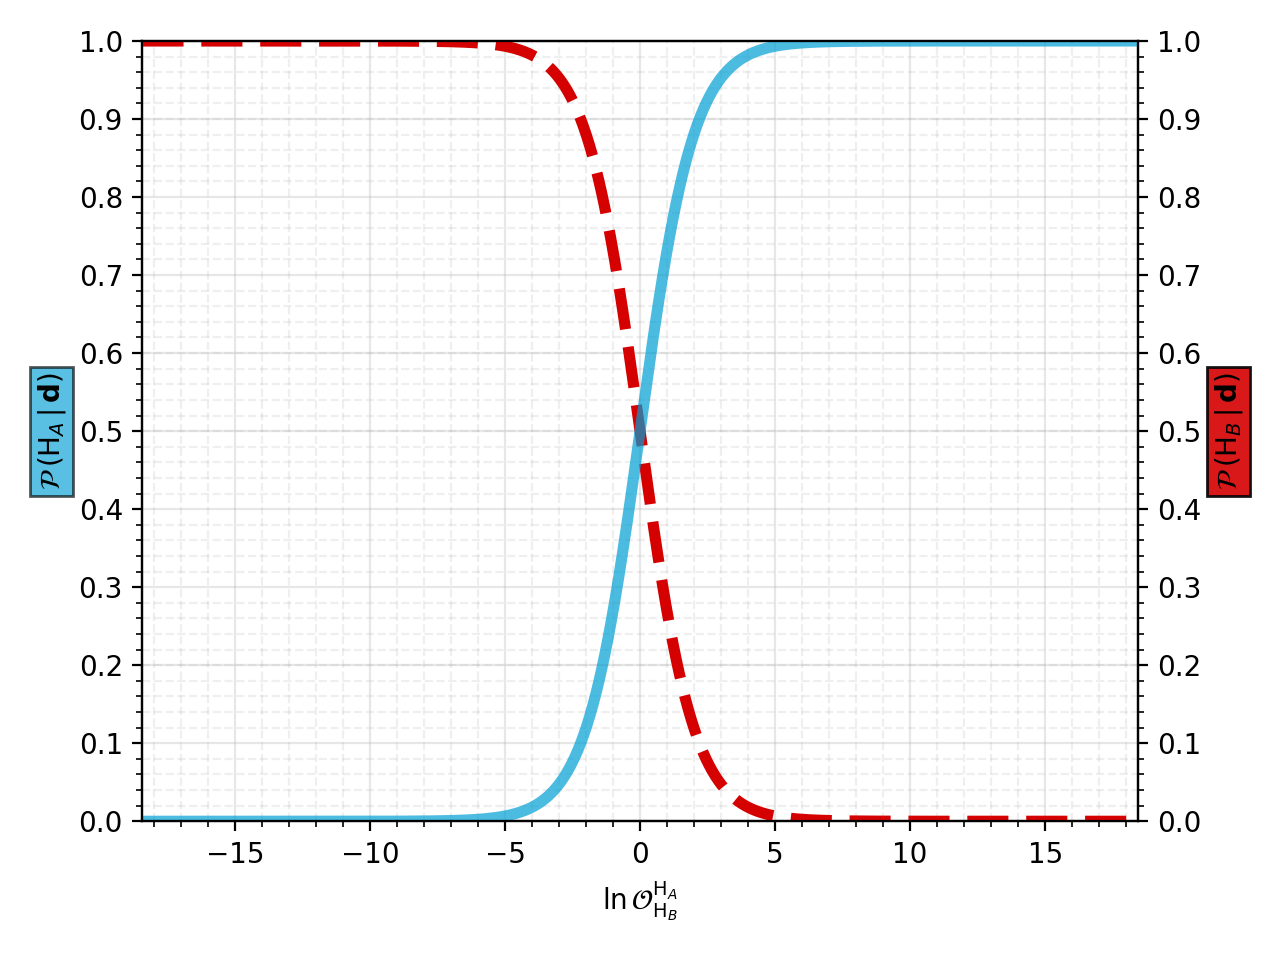
\includegraphics[width=\textwidth]{figs/chapter5/log_odds_probability.png}
  \caption{(\textit{Light blue, solid}) The probability of hypothesis $\mathrm{H}_A$ being favored over hypothesis $\mathrm{H}_B$ after observation of the data $\mathbf{d}$ when considering calculating the natural log of the odds ratio for each hypothesis. (\textit{Red, dashed}) The posterior probability of $\mathrm{H}_B$ is the complement of the posterior probability of $\mathrm{H}_A$ if there are only two hypotheses available to test. When $\mathrm{log}_{10} \; \mathcal{O} = 0$, the probability for each hypothesis is $50\%$.}
  \label{fig:log_odds_v_probability}
\end{figure}

\begin{figure}[th]
  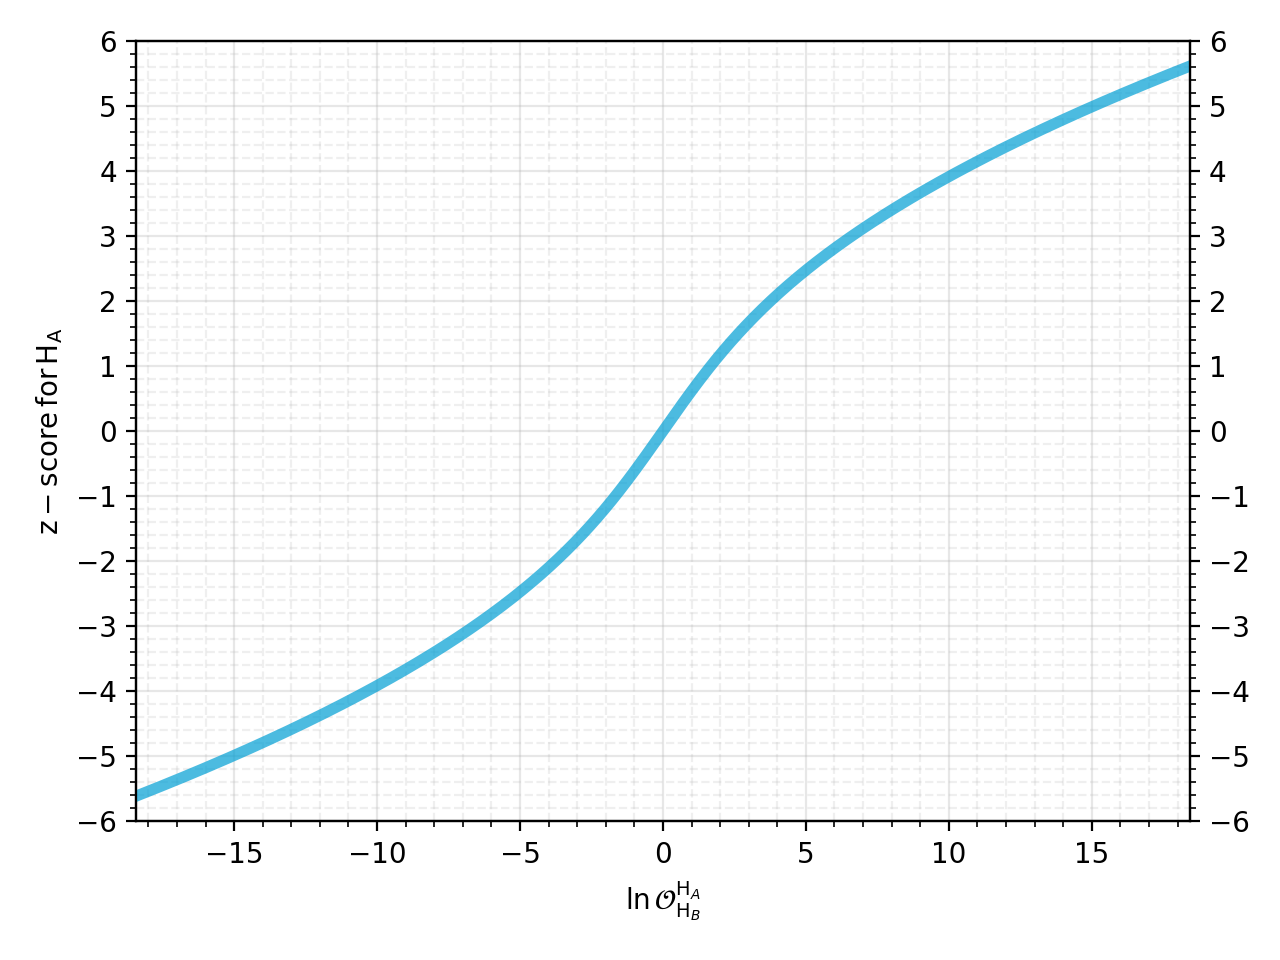
\includegraphics[width=\textwidth]{figs/chapter5/log_odds_z_score.png}
  \caption{The z-score pertaining to the same level of probability for  hypothesis 1 being favored over hypothesis 2 when considering the $\mathrm{ln} \, \mathcal{O}^{\mathrm{H}_A}_{\mathrm{H}_B}$. When $\mathrm{ln} \, \mathcal{O}^{\mathrm{H}_A}_{\mathrm{H}_B} = 0$, the z-score is $0 \sigma$ and the probability for each hypothesis is $50\%$. A z-score of $>5 \sigma$ has the same probability value as an odds ratio of $> 10^7$.}
  \label{fig:log_odds_v_z_score}
\end{figure}

\begin{figure}[th]
  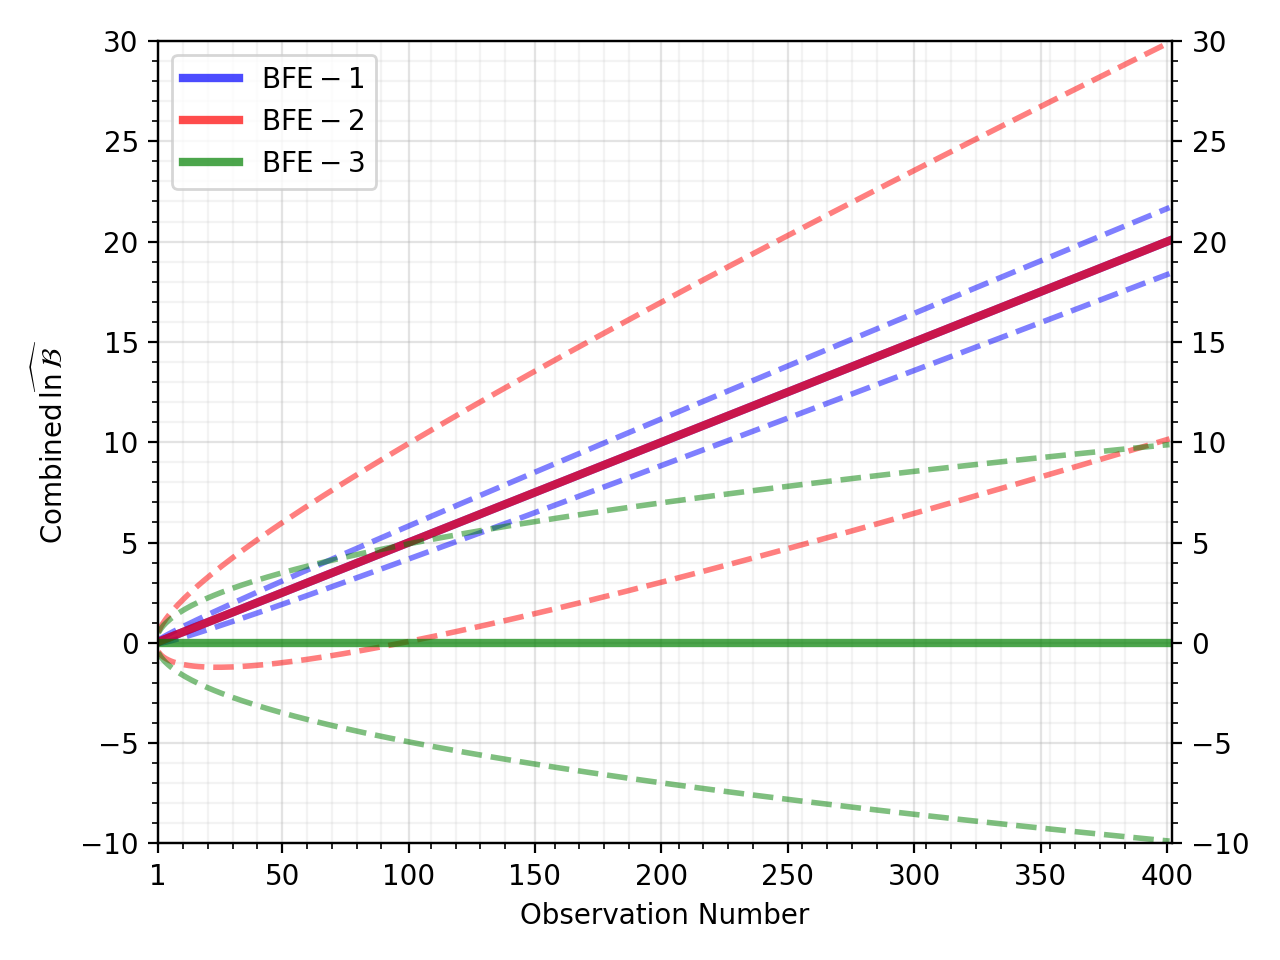
\includegraphics[width=\textwidth]{figs/chapter5/example_log_bf_divergence.png}
  \caption{The divergence of statistical inference for three hypothetical log Bayes factor estimators $\mathrm{E1}$, $\mathrm{E2}$, $\mathrm{E3}$ who are estimating the combined logarithm of the Bayes factor over many observations. Each observation has a true ln $\mathcal{B}$ of hypothesis $\mathrm{H}_A$ relative to $\mathrm{H}_B$ of $0.05$, indicating no statistical significance at the level of a single observation. Over $400$ events however the combined logarithm of the Bayes factor is $20$. The estimator $\mathrm{E1}$ (light blue) estimates the logarithm of the Bayes factor for each observation through an unbiased method, measuring a mean value of $\mu_i = 0.05$ for each observation with standard deviation $\sigma_i = 0.05$. The estimator $\mathrm{E2}$ (light red) estimates the logarithm of the Bayes factor for each observation through an unbiased method, measuring a mean value of $\mu_i = 0.05$ for each observation with a very large standard deviation $\sigma_i=0.3$. The estimator $\mathrm{E3}$ (light green) estimates the logarithm of the Bayes factor for each observation through a slightly biased method, instead measuring a mean value of $mu_i = 0$ for each observation but has a small measuring uncertainty of $\sigma_i=0.05$. The inferences of these estimators diverge after many observations due to systematic and statistical uncertainty.}
  \label{fig:LBFE}
\end{figure}


\begin{figure}[th]
\centering
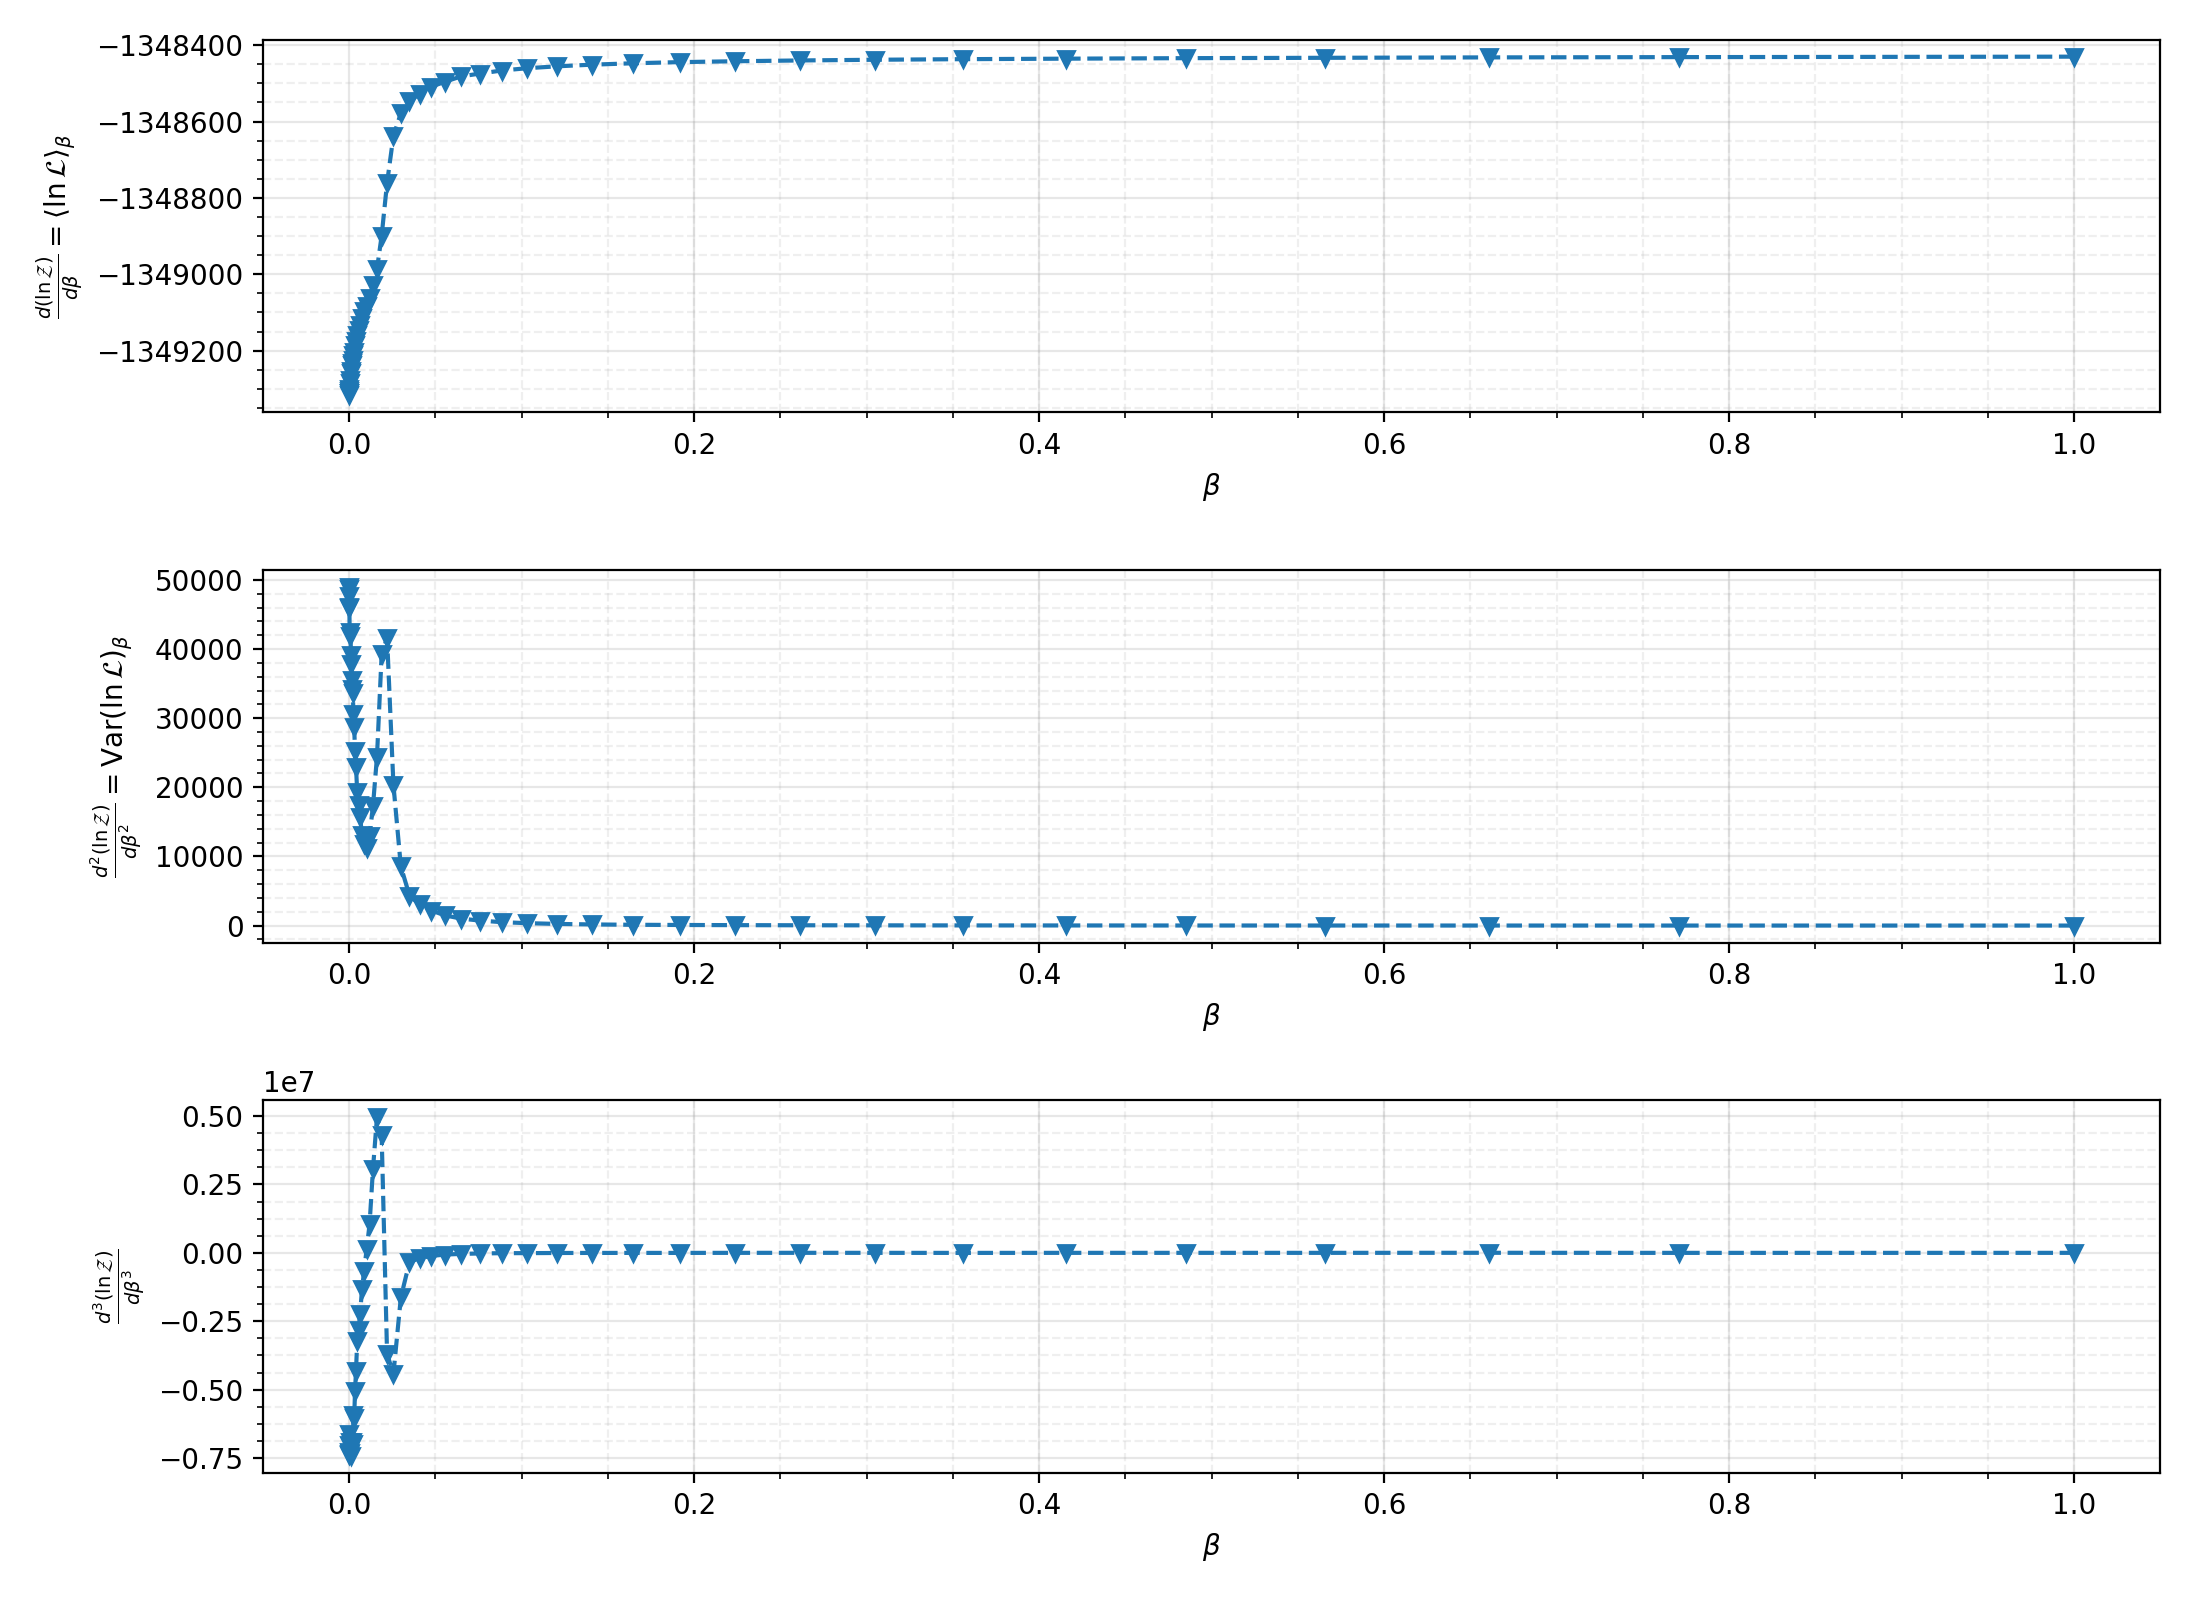
\includegraphics[width=1.0\textwidth]{figs/chapter6/gooseneck_plots_linear.png}
\caption{The subplots of the thermodynamic integrand and subsequent derivatives of the thermodynamic integral. (\textit{Top}) The thermodynamic integrand when compared to the inverse-temperature $\beta$. The curve should be smooth and montonic, however it is very difficult to inspect the integrand on a linear $\beta$ scale. (\textit{Middle}) The second derivative of the logarithm of the evidence is the variance of the power-posterior at an inverse temperature $\beta$. There is some indication that an inflection point happens in the curvature of the integrand at high temperature. (\textit{Bottom}) The third derivative of the logarithm of the evidence is also the third-order cumulant of the power-posterior distributions at an inverse-temperature $\beta$. It is difficult to inspect the behavior of this derivative on the linear $\beta$ scale.}
\label{fig:gooseneck_linear}
\end{figure}

\begin{figure}[th]
\centering
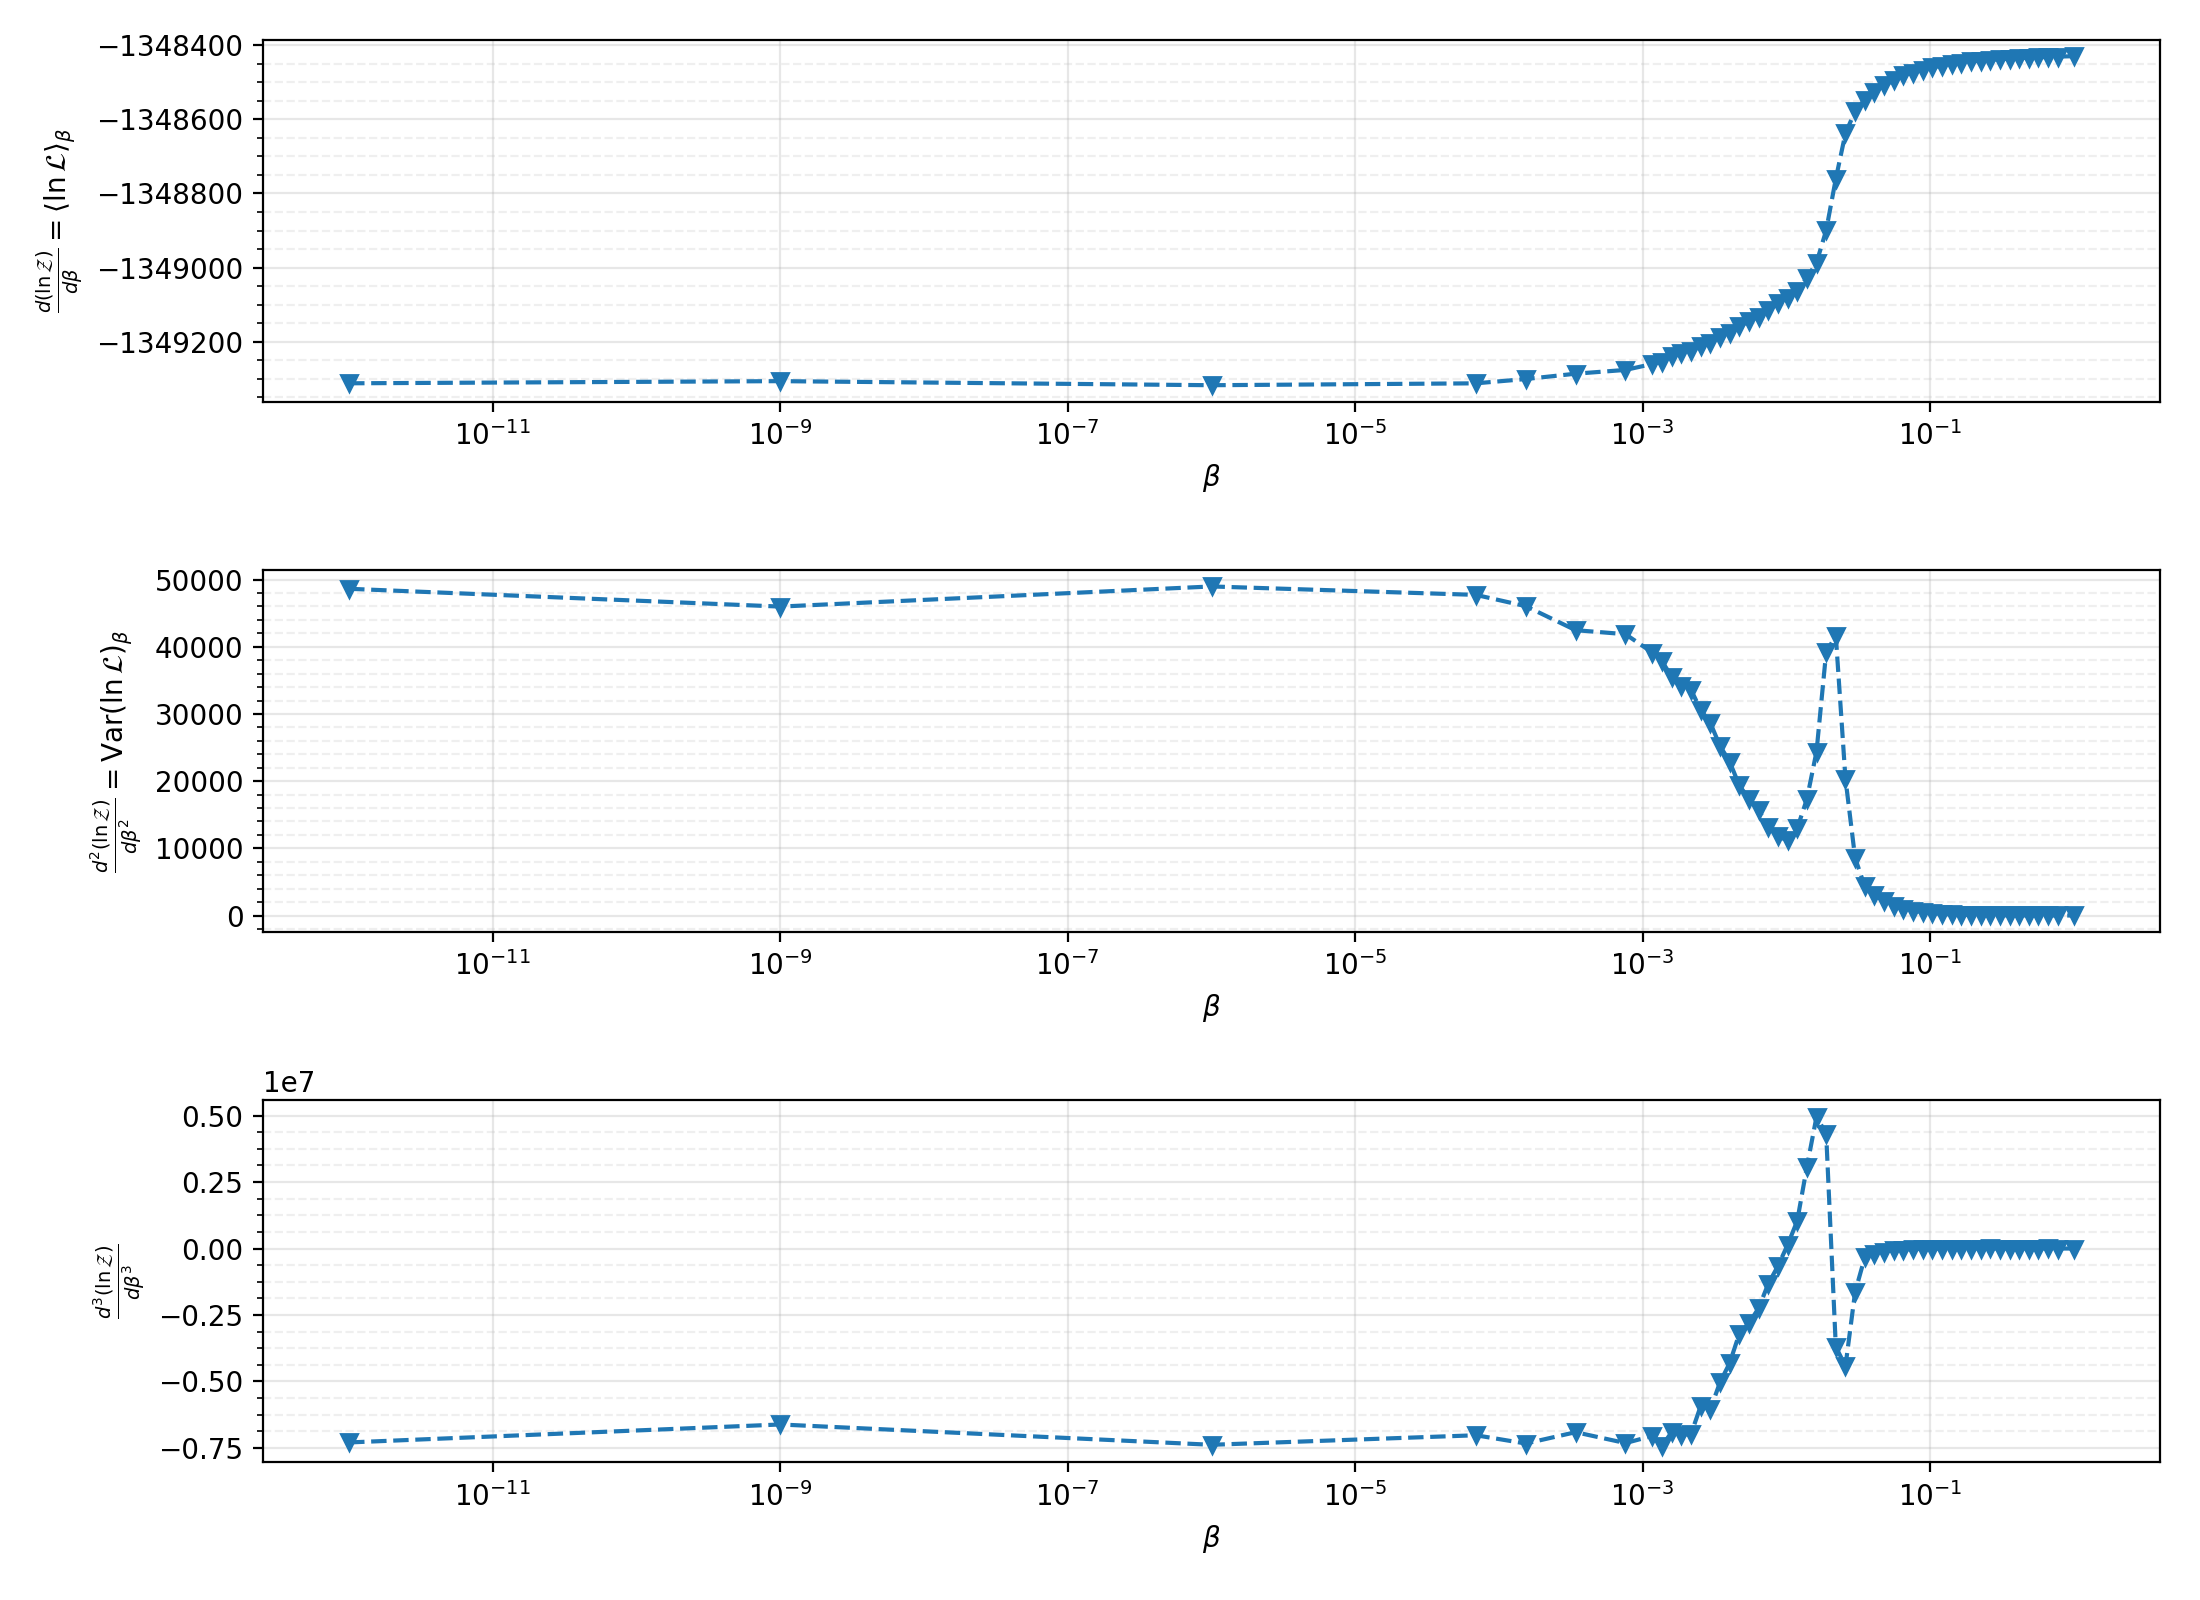
\includegraphics[width=1.0\textwidth]{figs/chapter6/gooseneck_plots_log.png}
\caption{The subplots of the thermodynamic integrand and subsequent derivatives of the thermodynamic integral. (\textit{Top}) The thermodynamic integrand when compared to the inverse-temperature $\beta$. The curve should be smooth and montonic, however there is some indication at $\beta = 10^{-9}$ that this condition is not strictly met in the Markov Chain Monte Carlo simulation. (\textit{Middle}) The second derivative of the logarithm of the evidence is the variance of the power-posterior at an inverse temperature $\beta$. This function should also be smooth however there is some indication that at high temperature that the derivatives are not stable. (\textit{Bottom}) The third derivative of the logarithm of the evidence is also the third-order cumulant of the power-posterior distributions at an inverse-temperature $\beta$. Here we can see that the derivatives are not very sable or smooth. This may motivate moving our analysis to new multi-tempered samplers that are optimized for thermodynamic integration.}
\label{fig:gooseneck_log}
\end{figure}

\begin{figure}[th]
\centering
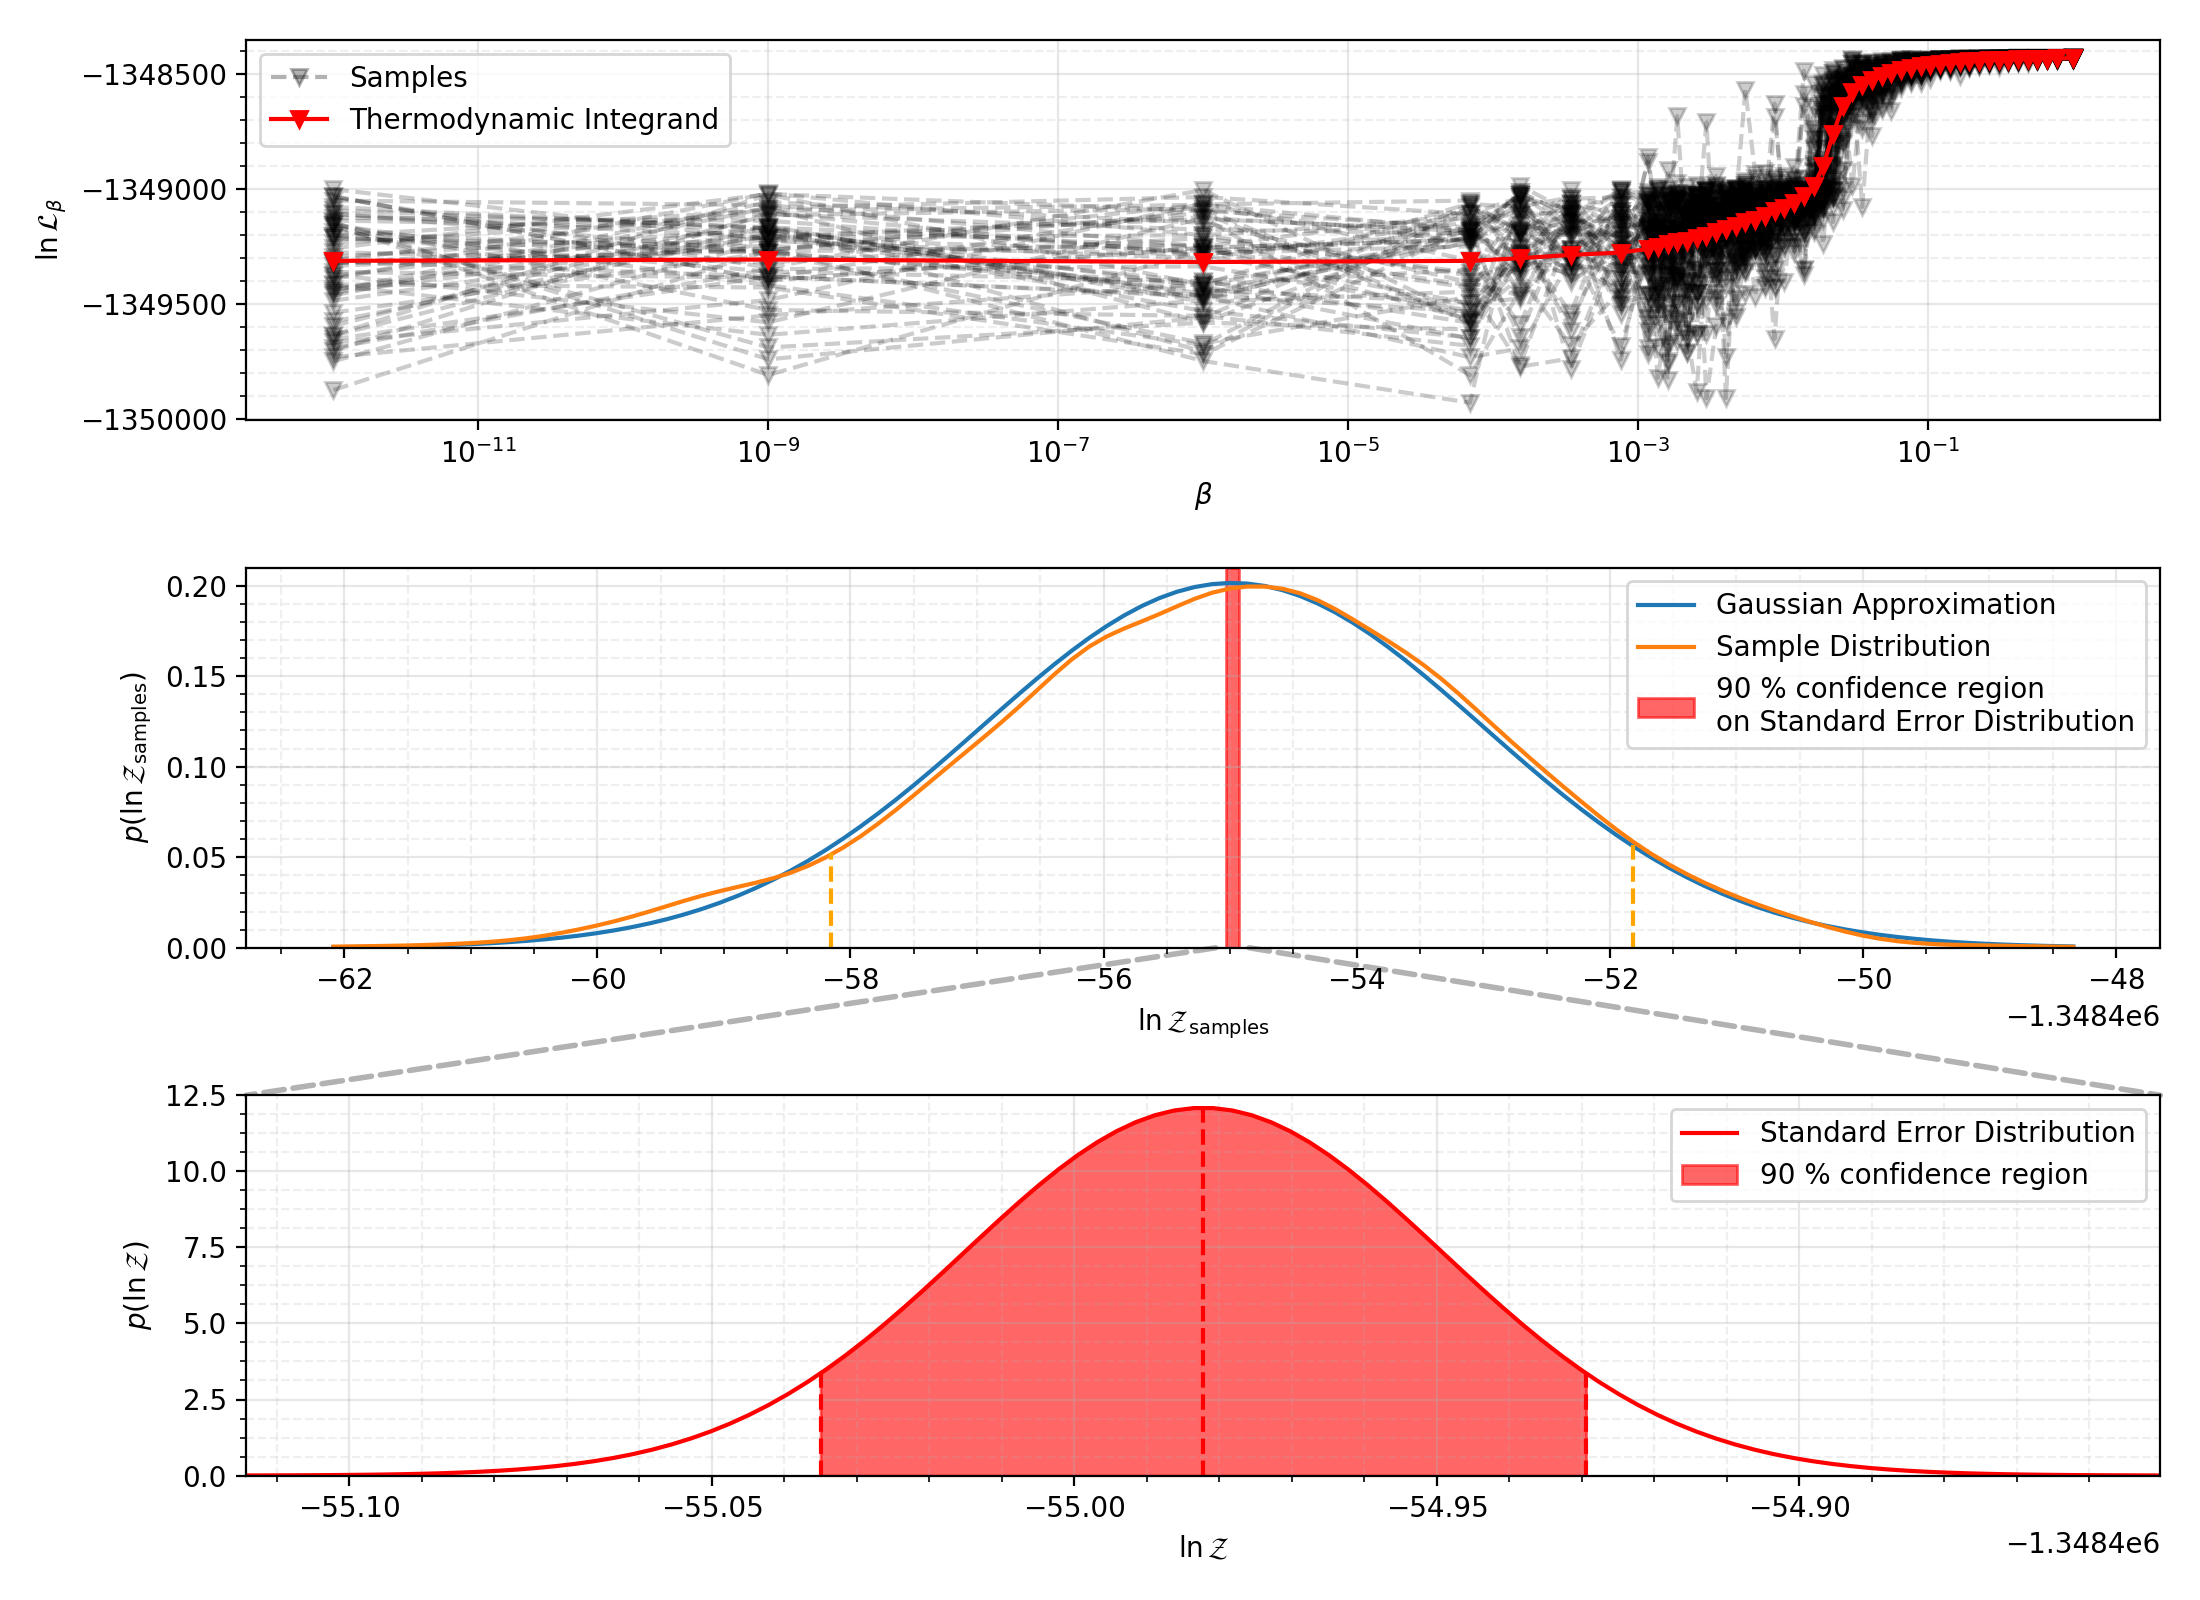
\includegraphics[width=1.0\textwidth]{figs/chapter6/ti_monte_carlo_error.png}
\caption{The first subplot denotes the untempered log-likelihood samples when drawn from the power-posteriors at $\beta$. The expectation value of the untempered log-likelihood when drawn from these power-posteriors is the thermodynamic integrand and is plotted in red. The thermodynamic integral over all geometric paths given from the samples is drawn in the second subplot. The sample-log-integral distribution is approximately a Gaussian distribution. The standard error of the mean value of the log evidence is given by the sample standard deviation divided by the square root of the number of samples. The $90 \%$ confidence interval on the sample distribution in the log-evidence is drawn in dashed orange lines. The $90\%$ confidence region from this standard error is shaded in red. The final subplot is a zoom-in on this $90 \%$ confidence region showing the error estimate on the thermodynamic integral due to Monte Carlo sampling.}
\label{fig:ti_monte_carlo_error}
\end{figure}

\begin{figure}[th]
\centering
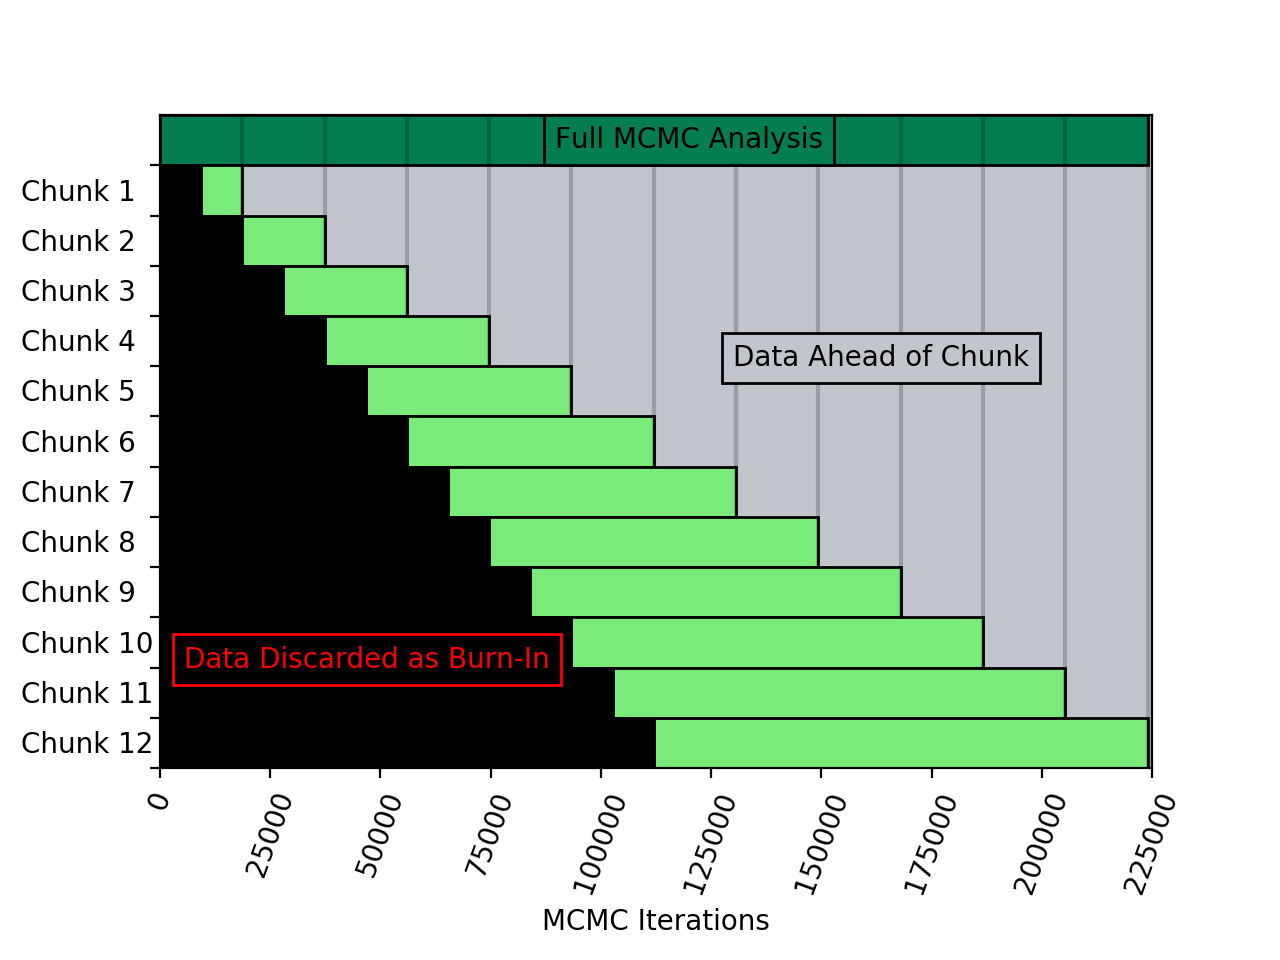
\includegraphics[width=1.0\columnwidth]{figs/chapter6/convergence_segmentation_lvc_sim.png}
\caption{The partitioning of the MCMC analysis to check on the convergence of the thermodynamic integrand and the thermodynamic integration. The dark-green bar at the top represents all of the samples collected by the MCMC analysis. This segment is divided into 12 segments represented by the light gray lines. The light-green segments represent chunks that independent samples can be drawn from. The dark region represents samples discarded as burn-in samples for the MCMC. The dark grey region represents data that is ahead of the chunk and thus not used in drawing independent samples for that chunk. Chunk $12$ produces the identical samples as drawing independent samples according to the $\mathrm{n_{acl}}$ algorithm from PyCBC at the end of the analysis.}
\label{fig:nacl_segments}
\end{figure}

\begin{figure}[th]
\centering
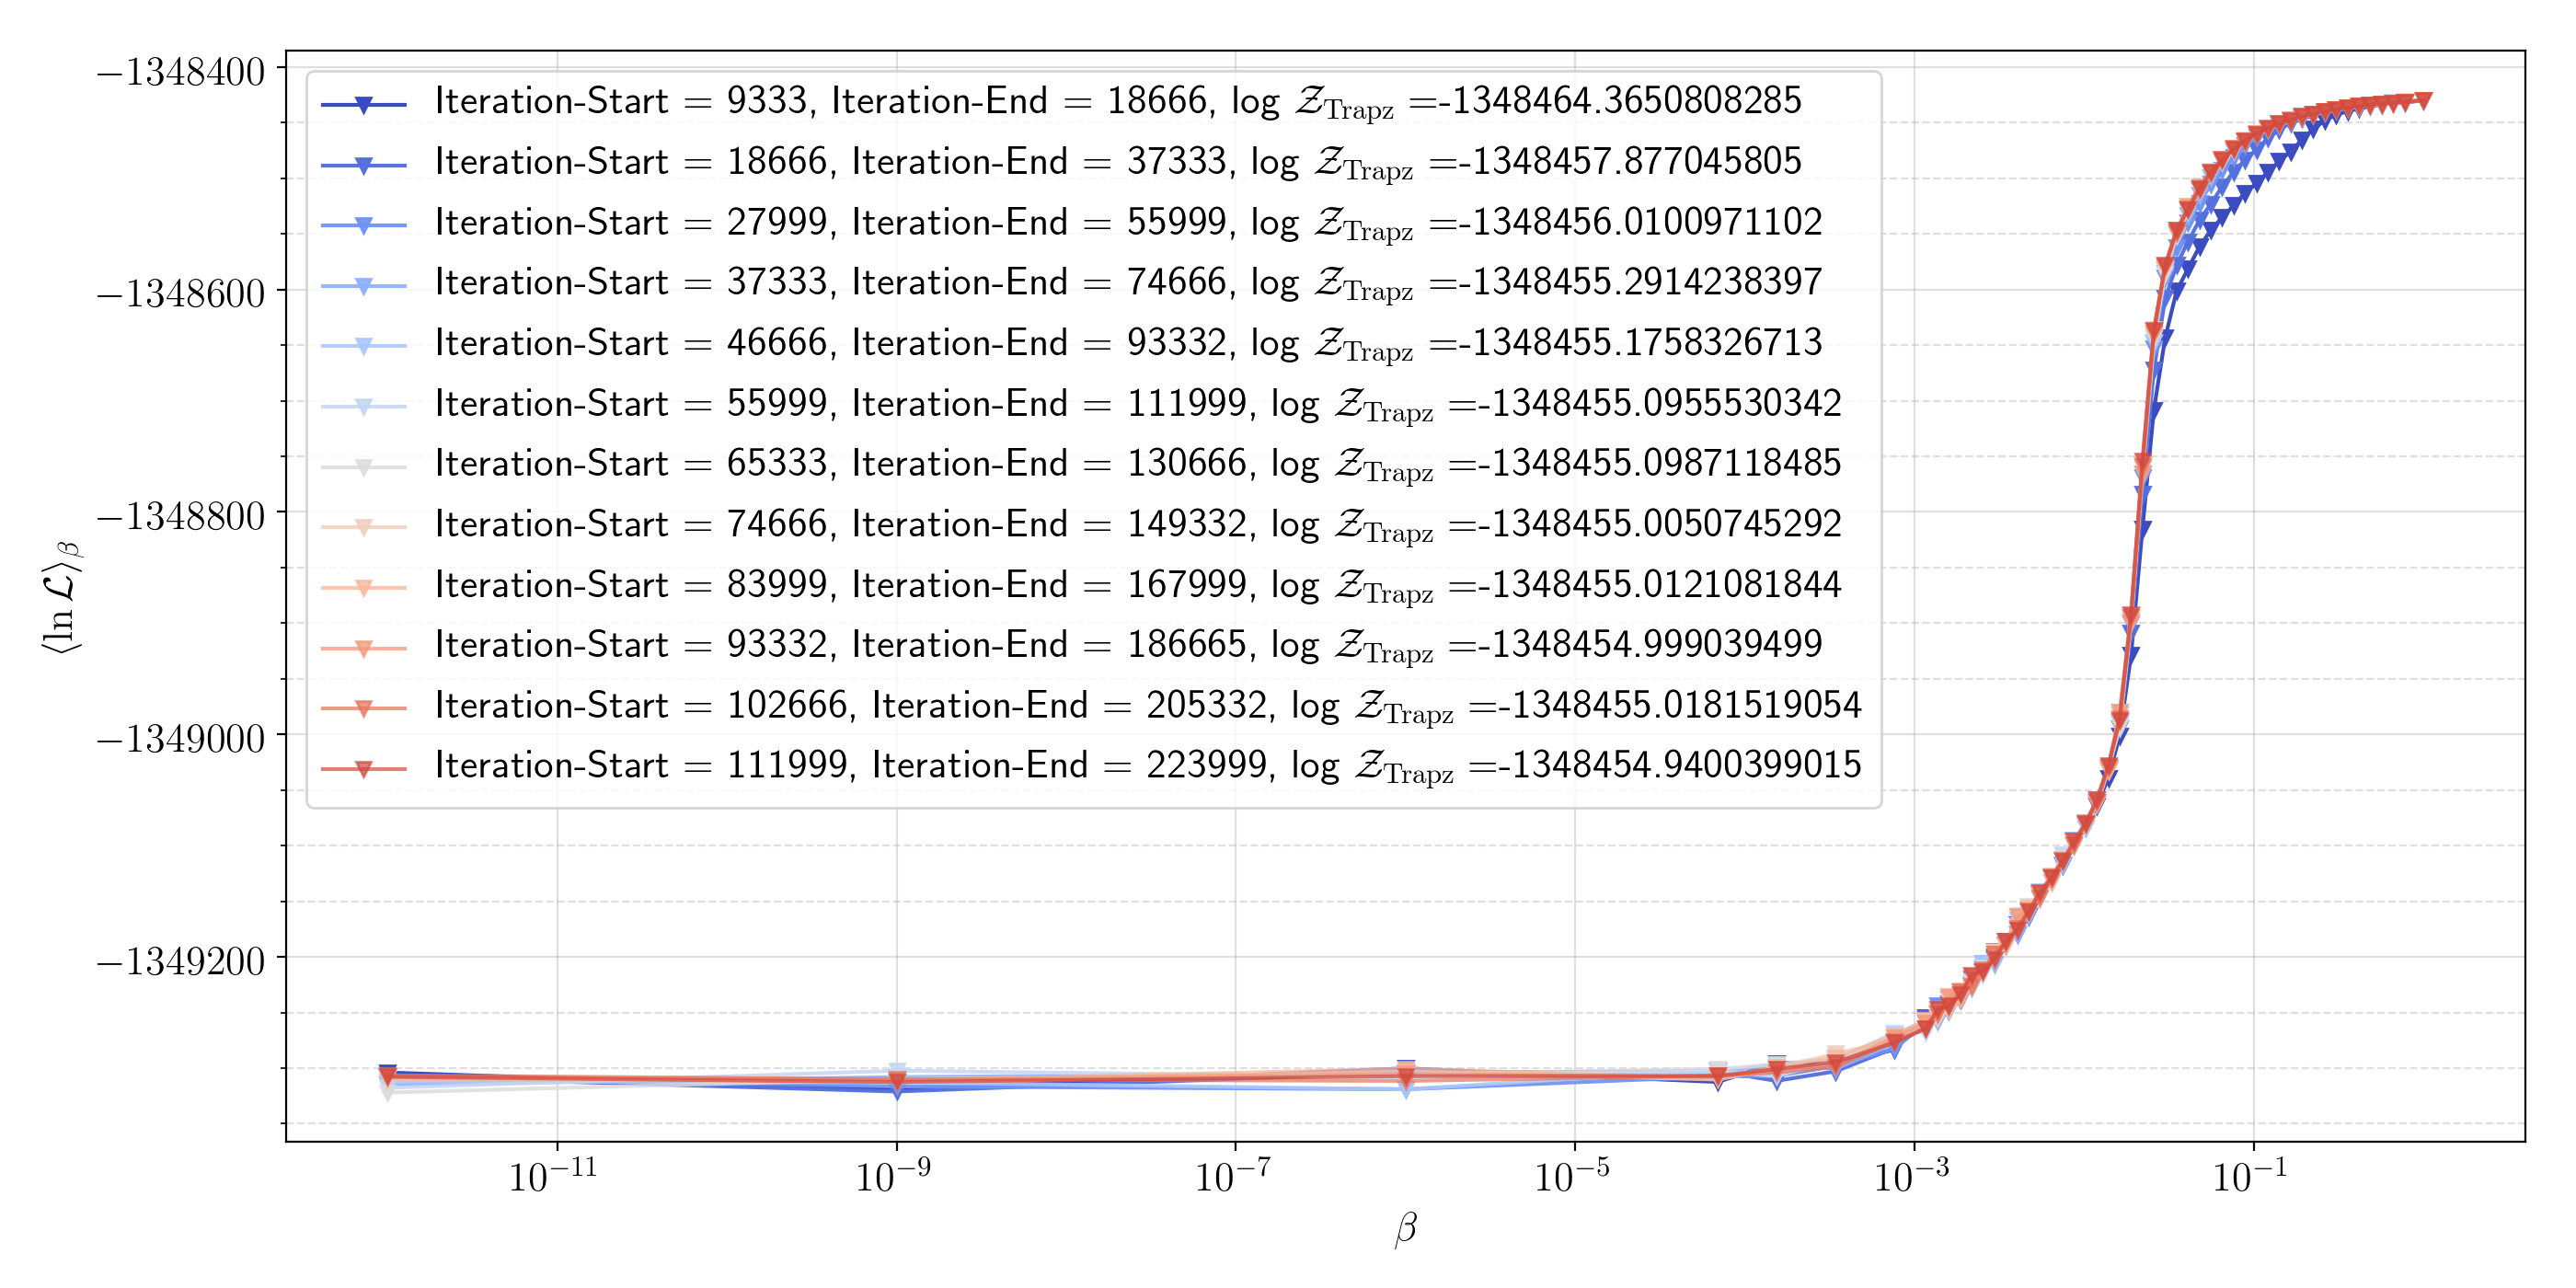
\includegraphics[width=1.0\columnwidth]{figs/chapter6/lsc_sim_integrand_progress.png}
\caption{The convergence of the thermodynamic integrand for a gravitational wave analysis using $51$ temperatures. This analysis neglected $\beta$ = $0$, but is otherwise an acceptable representation of the thermodynamic integrand. The Iteration-Start denotes the point is taken from a segment beginning with that MCMC iteration and ending with the MCMC iteration denoted as Iteration-End. These iterations correspond to the segments found in Fig.~\ref{fig:nacl_segments}. The logarithm of the evidence is shown also in the figure caption, and as the MCMC analysis progresses the integral converges to a set value. The thermodynamic integrand can be visually seen to converge to a S-like curve but the shape and curvature are unique to hypotheses and choice of data. Early in the MCMC analysis the thermodynamic integrand can be mishaped as the power-posteriors have not all converged. Experience has told us tha the power-posteriors that take the longest to converge tend to be in the region where the average log likelihood changes rapidly. Here this is in the region between $\beta$ $\in$ ($10^{-2} - 1$).}
\label{fig:integrand_convergence}
\end{figure}

\begin{figure}[th]
\centering
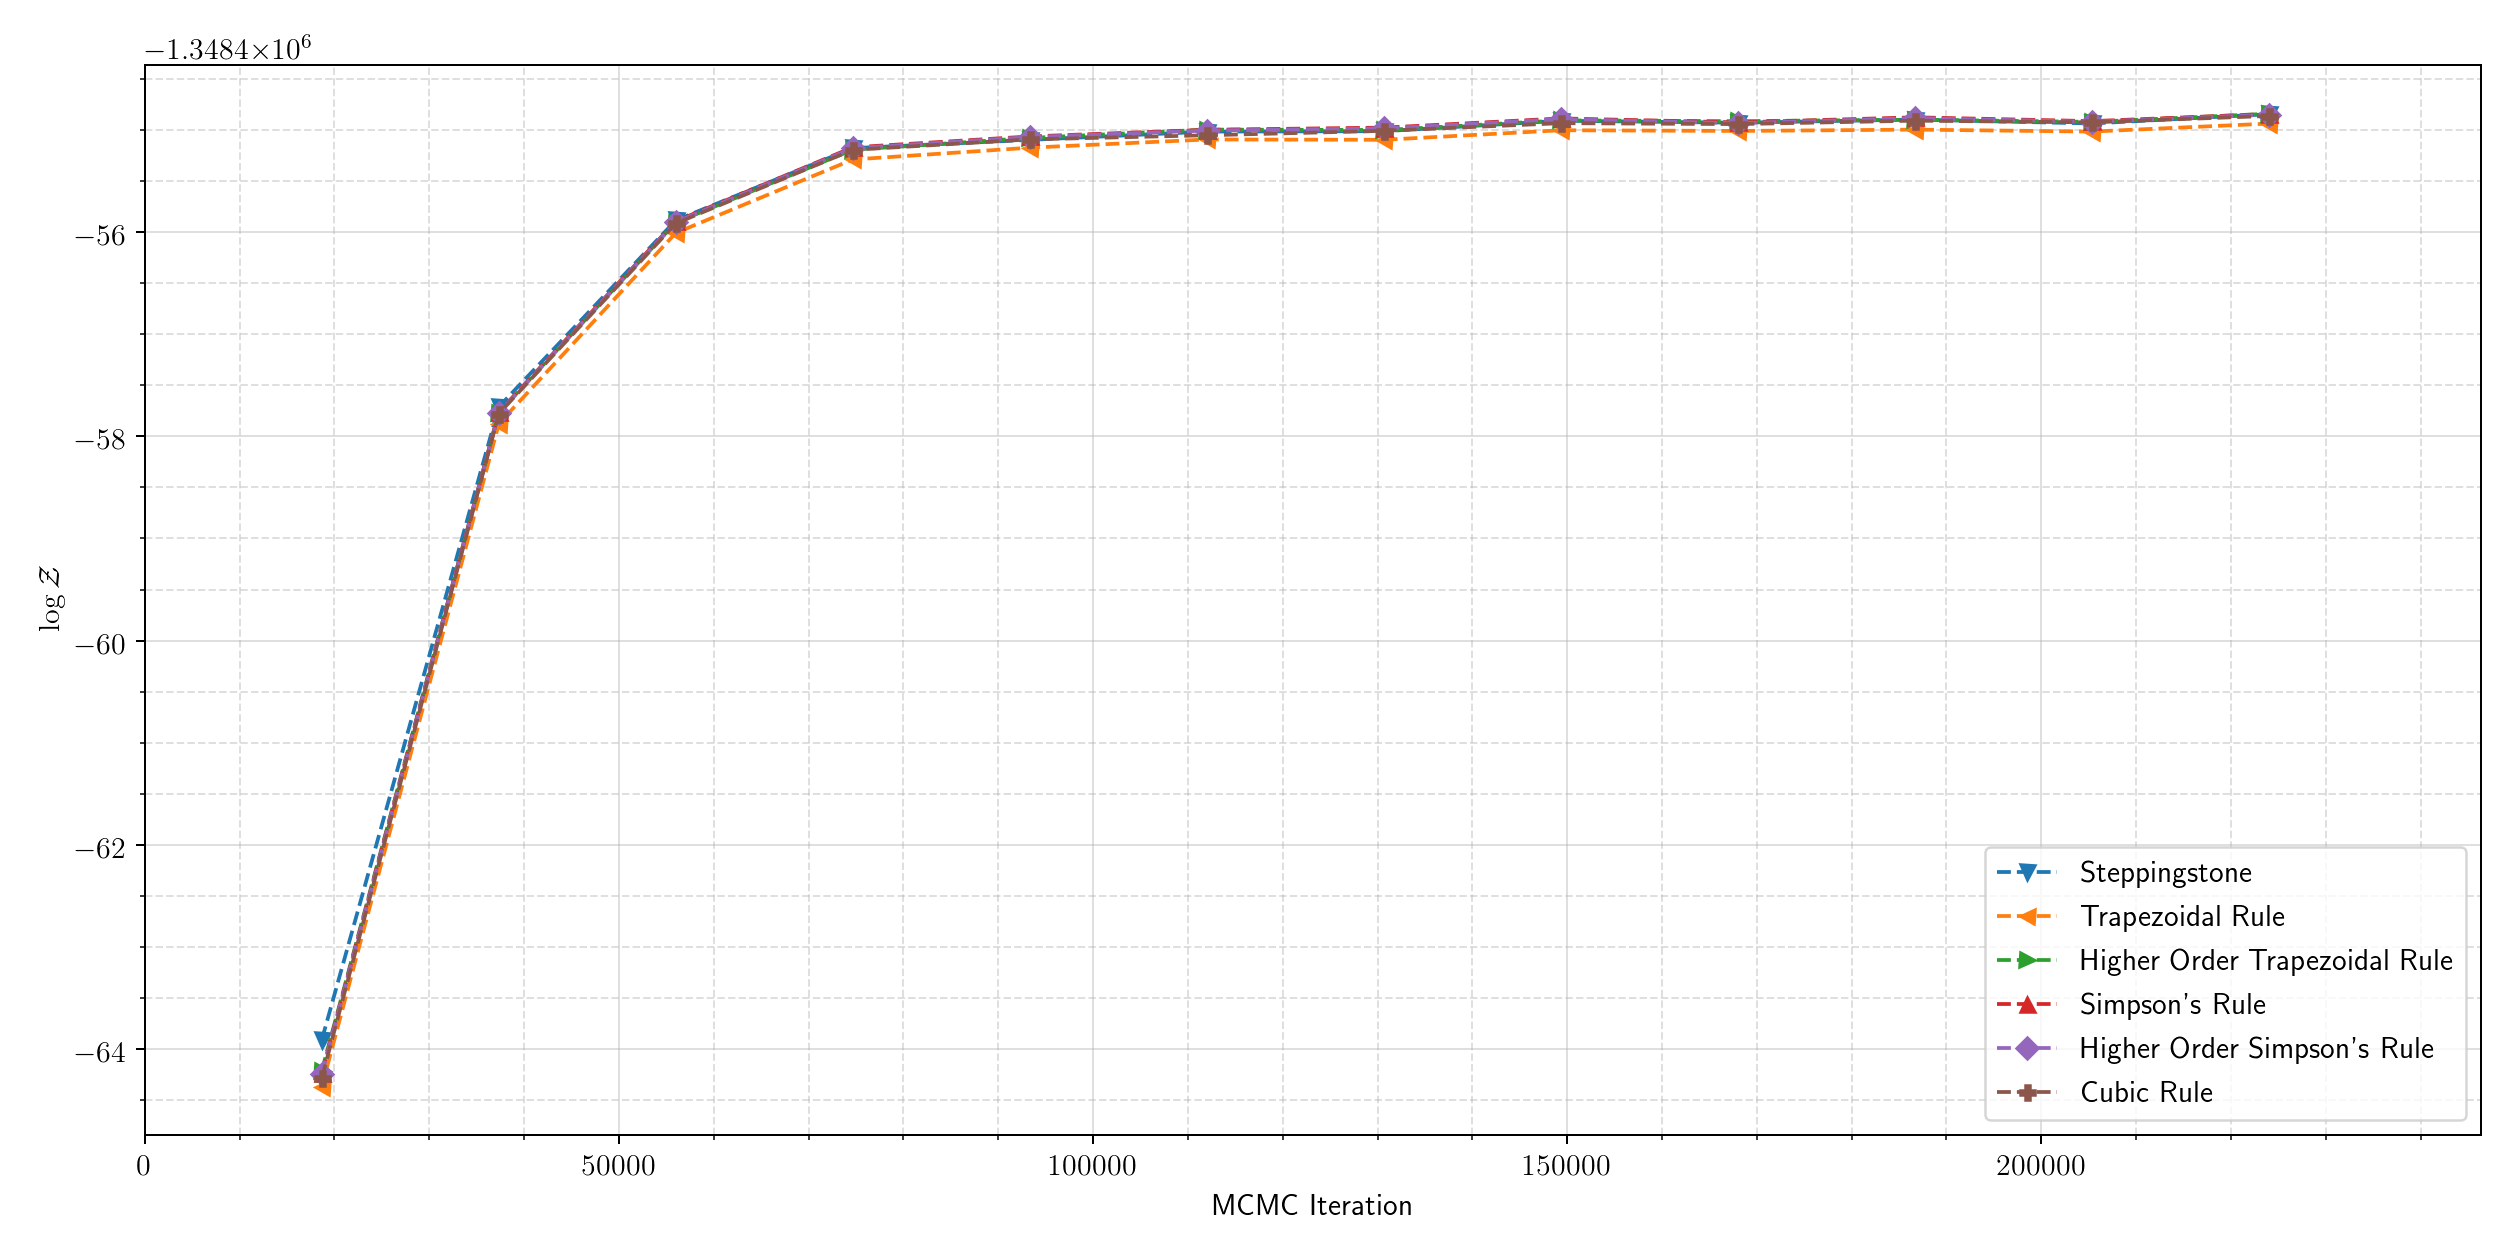
\includegraphics[width=1.0\columnwidth]{figs/chapter6/lvc_sim_evidence_convergence.png}
\caption{The convergence of the thermodynamic integral for a gravitational wave analysis using $51$ temperatures as a function of the MCMC iteration. These choice of points of iterations correspond to the segments found in Fig.~\ref{fig:nacl_segments}. As the analysis progresses the logarithm of the evidence from all quadrature methods tend towards a fixed value.}
\label{fig:integral_convergence}
\end{figure}

\newpage
\begin{sidewaystable}
\centering
\begin{tabularx}{1.0\textwidth}{c|c|c|c|c}
\hline\hline
Bayes factor & log Bayes factor & Posterior Probability & z-score & Interpretation \\
$\mathcal{B}^{\mathrm{H}_A}_{\mathrm{H}_B}$ & ln $\mathcal{B}^{\mathrm{H}_A}_{\mathrm{H}_B}$ & $\mathcal{P} \left(\mathrm{H}_A \, | \, \mathbf{d} \right)$ & $\sigma$ & - \\
\hline\hline
$2.7 \times 10^{-7}$ to $2.7 \times 10^{-5}$ & $-15.1$ to $-10.5$ & $2.7 \times 10^{-7}$ to $2.7 \times 10^{-5}$ & $-5$ to $-4$ & Very strong evidence for $\mathrm{H}_{B}$\\
$2.7 \times 10^{-5}$ to $0.0014$ & $-10.5$ to $-6.6$ & $2.7 \times 10^{-5}$ to $0.0014$ & $-4$ to $-3$ & Very strong evidence for $\mathrm{H}_B$ \\
$0.001$ to $0.022$ & $-6.6$ to $-3.8$ & $0.0014$ to $0.02$ & $-3$ to $-2$ & Strong evidence for $\mathrm{H}_B$ \\
$0.022$ to $0.18$ & $-3.8$ to $-1.7$ & $0.02$ to $0.15$ & $-2$ to $-1$ & Moderate evidence for $\mathrm{H}_B$ \\
$0.18$ to $1.0$ & $-1.7$ to $0$ & $0.15$ to $0.5$ & $-1$ to $0$ & Weak evidence for $\mathrm{H}_B$ \\
$1.0$ to $5.5$ & $0$ to $1.7$ & $0.5$ to $0.85$ & $\, 0$ to $\, 1$ & Weak evidence for $\mathrm{H}_A$ \\
$5.5$ to $45$ & $1.7$ to $3.8$ & $0.85$ to $0.98$ &  $\, 1$ to $\, 2$ & Moderate evidence for $\mathrm{H}_A$ \\
$45$ to $740$ & $3.8$ to $6.6$ & $0.98$ to $0.9986$ & $\, 2$ to $\, 3$ & Strong evidence for $\mathrm{H}_A$ \\
$740$ to $3.6 \times 10^{4}$ & $6.6$ to $10.5$ & $0.9986$ to $0.999972$ &  $\, 3$ to $\, 4$ & Very strong evidence for $\mathrm{H}_A$ \\
$3.6 \times 10^{4}$ to $3.6 \times 10^{6} $ & $10.5$ to $15.1$ & $0.999972$ to $0.99999972$ &  $\, 4$ to $\, 5$ & Very strong evidence for $\mathrm{H}_A$ \\
\hline\hline
\end{tabularx}
\caption{An empirical scale for evaluating the relative strength of evidence between hypothesis $\mathrm{H}_A$ and an alternative hypothesis $\mathrm{H}_B$ loosely adapted from Tables $1$ $\&$ $2$ of~\cite{trotta2008bayes}. We assume a prior odds ratio of unity between the two hypotheses, indicating no prior preference for either hypothesis. This makes the Bayes factor identical to the odds ratio and so we neglect the odds ratio here. Note that we have rounded to $2$ significant digits leaving a minor rounding discrepancy with Table~\ref{tab:results}. The interpretation column is only a rule of thumb and interpretations vary across scientific fields and experimental contexts.}\label{table:bayes_factor_interpretation}
\end{sidewaystable}


\newpage

\begin{sidewaystable}
\centering
\begin{tabularx}{1.0\textwidth}{c |c | c | c}
\hline\hline
Derivative & Result & Moment Representation & Cumulant \\
\hline\hline
\multirow{2}{*}{$\frac{d (\mathrm{ln} \, \mathcal{Z})}{d\beta}$} & \multirow{2}{*}{$\frac{\mathcal{Z}'}{\mathcal{Z}}$} & \multirow{2}{*}{$\langle \mathrm{ln} \, \mathcal{L} \rangle_\beta$} & \multirow{2}{*}{$\mu_1$} \\
 & & & \\
\hline
\multirow{2}{*}{$\frac{d^2 (\mathrm{ln} \, \mathcal{Z})}{d\beta ^2}$} & \multirow{2}{*}{$\frac{\mathcal{Z}''}{\mathcal{Z}} - \frac{\mathcal{Z}'^2}{\mathcal{Z}^2}$} & \multirow{2}{*}{$\langle (\mathrm{ln} \, \mathcal{L})^2 \rangle_\beta - \langle \mathrm{ln} \, \mathcal{L} \rangle^2_\beta$}  & \multirow{2}{*}{$\mu_2$ - $\mu_1^2$} \\
& & & \\
\hline
\multirow{2}{*}{$\frac{d^3 (\mathrm{ln} \, \mathcal{Z})}{d\beta ^3}$}  & \multirow{2}{*}{$\frac{\mathcal{Z}^{(3)}}{\mathcal{Z})}+ 2 \frac{\mathcal{Z}'^3}{\mathcal{Z}^3} -  3 \frac{\mathcal{Z}' \mathcal{Z}''}{\mathcal{Z}^2}$} &  \multirow{2}{*}{$\langle (\mathrm{ln} \, \mathcal{L})^3 \rangle_\beta  + 2 \langle \mathrm{ln} \, \mathcal{L} \rangle^3 - 3 \langle (\mathrm{ln} \, \mathcal{L})^2 \rangle_\beta \langle \mathrm{ln} \, \mathcal{L} \rangle_\beta$} & \multirow{2}{*}{$\mu_3 + 2\mu_1^3 - 3\mu_2 \mu_1$}  \\
& & & \\
\hline
\multirow{5}{*}{$\frac{d^4 (\mathrm{ln} \, \mathcal{Z})}{d\beta ^4}$} & \multirow{5}{*}{$\frac{\mathcal{Z}^{(4)}}{\mathcal{Z}} - 3 \frac{\mathcal{Z}''^2}{\mathcal{Z}^2} - 6 \frac{\mathcal{Z}'^4 }{\mathcal{Z}^4} - 4 \frac{\mathcal{Z}^{(3)} \mathcal{Z}'}{\mathcal{Z}^2} + 12 \frac{\mathcal{Z}'^2 \mathcal{Z}''}{\mathcal{Z}^3}$} & \multirow{5}{*}{\begin{multlined} $\langle (\mathrm{ln} \, \mathcal{L})^4 \rangle_\beta - 3 \langle (\mathrm{ln} \, \mathcal{L})^2 \rangle^2_\beta - 6 \langle \mathrm{ln} \, \mathcal{L} \rangle_\beta^4$ \\ $- 4 \langle (\mathrm{ln} \, \mathcal{L})^3 \rangle_\beta \langle \mathrm{ln} \, \mathcal{L} \rangle_\beta + 12 \langle (\mathrm{ln} \, \mathcal{L} )^2 \rangle_\beta \langle \mathrm{ln} \, \mathcal{L} \rangle^2_\beta$ \end{multlined}} & \multirow{5}{*}{\begin{multlined}$\mu_4 - 3 \mu_2^2 - 6 \mu_1^4$ \\ - $4\mu_3\mu_1 + 12\mu_2\mu_1^2$\end{multlined}} \\
 & & & \\
 & & & \\
 & & & \\
 & & & \\
\hline\hline
\end{tabularx}
\caption{The table of derivatives of the thermodynamic integral along with the moment representation of the derivatives of the thermodynamic integral and a set of reference of cumulants~\cite{kardar2007statistical}. The cumulants are represented in terms of the non-central moments of a distribution so that the representation is made clear with the moment representation of the derivatives of the thermodynamic integral. The non-central moment $\mu_i$ represents the expectation value $\langle x^i\rangle$, where $x$ is the one dimensional independent variable of a probability distribution function~\cite{abramowitz1965handbook}. We only present four derivatives of the thermodynamic integral for both brevity and because our data are typically not accurate enough to estimate higher order cumulants. We have inspected that this relation holds up to the $7$th derivative. Further orders could also be checked, although a formal proof may be more satisfactory.} \label{table:cumulants}
\end{sidewaystable}

